\chapter{Графы}

%graph: label prefix
История графов началась с головоломок. Первым упоминанием считается 1736 г., когда Леонард Эйлер решил задачу о Кёнигсбергских мостах, используя граф.
\begin{exampl}[Задача о Кёнигсбергских мостах]
    Река Прегель (Преголя) делила Кёнигсберг на четыре главные части: Альтштадт ($A$), Форштадт ($B$), Кнайпхоф ($C$) и Ломзе ($D$). Части соединены друг с другом семью мостами (см. рис. \ref{fig:graph:kenigsberg}). Возможно ли составить такой маршрут, чтобы пройти по каждому мосту только один раз и вернуться в исходную точку?    
\end{exampl}
\begin{proof}[Решение]
    Критерий возможности построения такого маршрута приведен в разделе \ref{sctn:graph:cycles}.
\end{proof}

Эйлер свел задачу к графу и вывел правило определения возможен ли подобный обход в общем случае.
\begin{figure}
    \centering
    \begin{tabular}{cc}
        \fbox{
            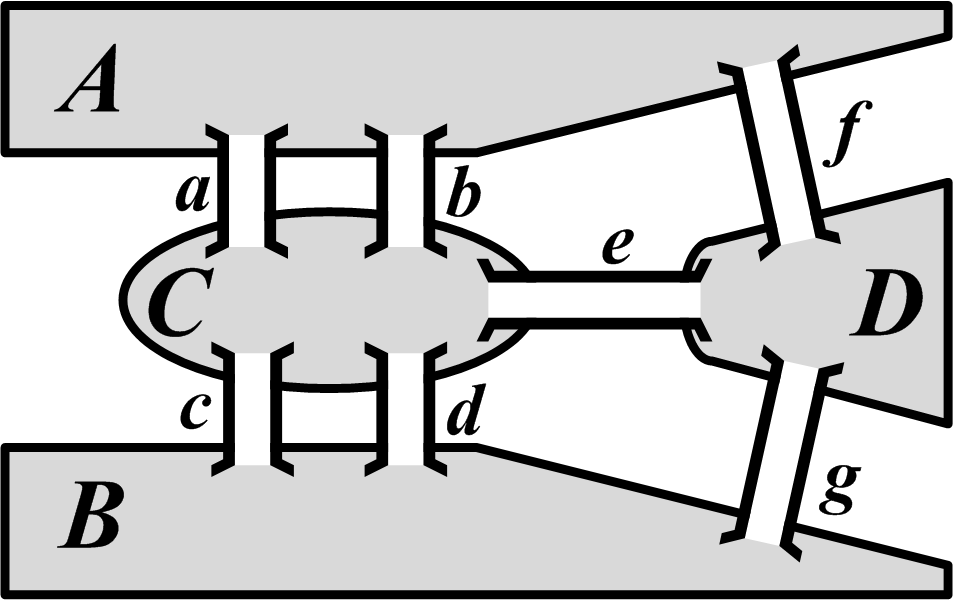
\includegraphics[width=0.3\textwidth]{fig/kenigsberg.png}
        }
        &
        \(
            {\xymatrix{
                A \ar@{-}@/^/[d]^b \ar@{-}@/_/[d]_a \ar@{-}@/^/[dr]^f
                    &*{}
                        \\
                C \ar@{-}[r]^e
                    &D
                        \\
                B \ar@{-}@/^/[u]^c \ar@{-}@/_/[u]_d \ar@{-}@/_/[ur]_g
                    &*{}
            }}
        \)        
    \end{tabular}
    \caption{Задача о Кенигсбергских мостах}
    \label{fig:graph:kenigsberg}
\end{figure}


Ныне теория графов --- это один из важнейших разделов дискретной математики, находящий массу практических применений в первую очередь из за своей наглядности. Графами моделируются схемы дорог, электрические схемы, химические соединения, схемы управления, автоматы, отношения и т.д. Для углубленного изучения теории графов можно рекомендовать книги: \cite{bib:shaporev:discretemath, bib:gorbatovs:discrmath, bib:novic:discrmathprogrammer}. Свободное изложение основ теории графов можно найти в книге \cite{bib:ore:graphs}.


\section{Основные термины и определения}

Граф $G$ --- это совокупность $G=\langle V,P\rangle$ \emph{множества} вершин $V$ и \emph{набора} отрезков $P$, соединяющих пары вершин. Отдельный отрезок представлен упорядоченной $(a,b)$ (или неупорядоченной $[a,b]$) парой, где $a,b\in V$. В общем случае, в наборе $P$ могут присутствовать несколько одинакового вида пар $(a,b)$.

Отрезок $[a,a]$, соединяющий вершину $a$ с ней самой, называется \emph{петлей}.

Неупорядоченная пара вершин $[a,b]$ (т.е. $[a,b]=[b,a]$) называется \emph{ребром}, а граф, содержащий только ребра называется \emph{неориентированным}.

Упорядоченная пара вершин $(a,b)$ (т.е. $(a,b)\neq(b,a)$) называется \emph{дугой}, а граф, содержащий только дуги называется \emph{ориентированным} или \emph{орграфом}. Дуга изображается стрелкой.

Если набор $P$ содержит несколько одинаковых отрезков-пар, то такие пары называются \emph{кратными}, а граф называется \emph{мультиграфом}.

Если задана функция $f:V\to M$ и/или $f:P\to M$, то множество $M$ называтется множеством \emph{пометок}, а граф называется \emph{помеченным}\footnote{Граф на рисунке \ref{fig:graph:kenigsberg} --- помеченный} (или \emph{нагруженным}). Пометка на изображении графа пишется над соответствующей вершиной или отрезком. Если пометка представляет собой число (или элемент упорядоченного множества), то она называется \emph{весом}, а граф --- \emph{взвешенным}.

Вершины, соединенные одним ребром, называются \emph{смежными}. Ребра, имеющие общую вершину, также называются \emph{смежными}. Ребро \emph{инцидентно} вершинам, которые оно соединяет, и вершины также \emph{инцидентны} этому ребру.

\emph{Степенью} вершины называется число ребер, инцидентных этой вершине. В орграфах различают полустепени исхода (количество исходящих дуг) и захода (количество входящих дуг).

Граф называется \emph{полным}, если между любыми его вершинами существует ребро. В полном графе с $n$ вершинами число ребер $m=\frac{n(n-1)}{2}$. \emph{Дополнение} графа до полного содержит все ребра полного графа, не принадлежащие исходному графу.

\emph{Подграфом} называется граф, в который входит лишь часть вершин исходного графа и часть его ребер, эти вершины соединяющих.

Последовательность 
\begin{equation}
    \label{eq:graph:path}
    v_1,p_1,v_2,p_2,\ldots,p_{n},v_{n+1},
\end{equation}
где $v_1,v_2,\ldots,v_{n+1}\in V$, $p_1,p_2,\ldots,p_{n}\in P$ и любые два соседних элемента инцидентны (т.е. $p_i=(v_i,v_{i+1}), 1\leq i\leq n$) называется \emph{$(v_1,v_{n+1})$-маршрутом}. $n$ --- число отрезков $p_i$ маршрута называется его \emph{длиной}.

Если все отрезки маршрута (кроме, возможно $p_1$ и $p_{n-1}$) различны, то он называется \emph{цепью}. Если все вершины маршрута (кроме, возможно $v_1$ и $v_{n+1}$) различны (а значит и отрезки), то маршрут называется \emph{простой} цепью.

Замкнутая ($v_1=v_n$) цепь называется \emph{циклом}. Замкнутая простая цепь называется \emph{простым} циклом.

В орграфе цепь называется \emph{путем}, а цикл --- \emph{контуром}.


\section{Способы задания графов}

Существует множество способов задать граф (см. рис. \ref{fig:graph:representation}):
\begin{itemize}
    \item аналитически;
    \item матрицей инцидентности;
    \item матрицей смежности;
    \item списком смежности.
\end{itemize}

\begin{figure}
    \centering

    \begin{tabular}{|c|c|c|}
        \hline
        &&\\
        {\xymatrix{
            a \ar@{->}[r]^2
                &b
                    \\
            c \ar@{->}[r]_5 \ar@{->}[ur]^3 \ar@{->}[u]^1
                &d \ar@{->}[u]_4
        }}
        &
        \raisebox{-.5\height}{
            \(
                \begin{array}{c|cccc}
                     &a&b&c&d\\\hline
                    a&0&1&0&0\\
                    b&0&0&0&0\\
                    c&1&1&0&1\\
                    d&0&1&0&0
                \end{array}
            \)
        }
        &
        \raisebox{-.5\height}{
            \(
                \begin{array}{c|ccccc}
                      & 1 & 2& 3& 4& 5\\ \hline 
                    a & -1& 1& 0& 0& 0\\
                    b & 0 &-1&-1&-1& 0\\
                    c & 1 & 0& 1& 0& 1\\
                    d & 0 & 0& 0& 1&-1
                \end{array}
            \)
        }
        \\ \cline{2-3}
        &\multicolumn{2}{|c|}{
        \(
            \{a\mapsto\{b\},b\mapsto\emptyset,
            c\mapsto\{a,b,d\},d\mapsto\{b\}\}
        \)
        }
        \\ \hline
    \end{tabular}
    \caption{Способы задания графов}
    \label{fig:graph:representation}
\end{figure}

Граф $G=\langle V,P\rangle$ можно задать аналитически, перечислив множество вершин $V$ и набор отрезков $P$.

Пусть $n=|V|$ --- количество вершин, а $m=|P|$ --- количество отрезков. 

Элементы \emph{матрицы инцидентности} $[G]_{n\times m}$ неориентированного графа определяются так:
\[
    [G]_{i,j}=
    \begin{cases}
        1, &\text{если вершина $v_i\in V$ инцидентна ребру $p_j\in P$},\\
        0, &\text{в противном случае.}
    \end{cases}
\]

В каждом $j$-м столбце матрицы по две $1$, если $p_j$ не петля, и одна в противном случае. 

Для орграфа элементы \emph{матрицы инцидентности} $[G]_{n\times m}$ определяются так:
\[
    [G]_{i,j}=
    \begin{cases}
         1, &\text{если вершина $v_i\in V$ --- начало дуги $p_j\in P$},\\
        -1, &\text{если вершина $v_i\in V$ --- конец дуги $p_j\in P$},\\
         0, &\text{в противном случае.}
    \end{cases}
\]

\emph{Матрица смежности вершин} $[G]_{n\times n}$:
\[
    [G]_{i,j}=
    \begin{cases}
         1, &\text{если $(v_i,v_j)\in P$},\\
         0, &\text{в противном случае.}
    \end{cases}
\]

Для мультиграфа вместо $1$ указывается количество кратных отрезков $(v_i,v_j)$.

Для представления графов в компьютерах наиболее часто используется \emph{список смежности вершин} 
\[
    \{v\mapsto \{v_s|v_s\in V,(v,v_s)\in P\}|v\in V\},
\]
для каждой вершины $v$ определяющий множество смежных с ней вершин $v_s$.

Не следует забывать, что орграф задает бинарное отношение, а потому часть способов задания графа уже была рассмотрена в главе \ref{ch:rel:rel}.


\section{Связность}

\emph{Связным} называется граф, в котором любые две вершины соединены цепью. Максимальный по количеству вершин связный подграф графа называется его \emph{компонентой связности}. Граф называется \emph{несвязным}, если число его компонент связности больше одной. 

Для ориентированного графа вводится понятие \emph{сильной} связности: в таком орграфе любые две вершины соединены двумя путями: путем с началом в первой вершине, и путем с началом во второй.

\emph{Число вершинной связности} графа --- это наименьшее число вершин, удаление которых в связном графе приводит несвязному графу. \emph{Число реберной связности} графа --- это наименьшее число ребер, удаление которых в связном графе приводит несвязному графу.

\begin{exampl}
    \label{ex:graph:net}
    Рассмотрим сеть передачи данных, состоящую из узлов (компьютеров) и каналов передачи информации между ними. Эту сеть легко представить графом, вершины которого соответствуют узлам, а ребра --- каналам передачи информации. Сеть исправна, если любая пара узлов способна обмениваться информацией. Надежность (живучесть) сети --- способность функционировать при выходе из строя одного или нескольких узлов и(или) каналов. Допустим, имеется сеть следующей структуры:
    \[
        {\xymatrix{
            n_1 \ar@{-}[dd]_{c_{1,2}} \ar@{-}[dr]^{c_{1,3}}
                &*{}
                    &n_5 \ar@{-}[d]_{c_{5,6}} \ar@{-}[r]^{c_{5,8}}
                        &n_8
                            \\
            *{}
                &n_3 \ar@{-}[d]^{c_{3,4}} \ar@{-}[r]^{c_{3,6}}
                    &n_6 \ar@{-}[ur]_{c_{6,8}} \ar@{-}[dr]^{c_{6,9}} \ar@{-}[d]_{c_{6,7}}
                        &*{}
                            \\
            n_2 \ar@{-}[r]_{c_{2,4}}
                &n_4
                    &n_7 \ar@{-}[r]_{c_{7,9}}
                        &n_9
                            \\
        }}
    \]
    где $n_i$ --- $i$-й узел, а $c_{i,j}$ --- канал, соединяющий $i$-й и $j$-й узлы.
    
    Если выйдет из строя канал $c_{1,2}$, то узлы $n_1$ и $n_2$ не смогут обмениваться информацией непосредственно, но они могут передавать информацию маршрутом: 
    \[c_{1,3},n_3,c_{3,4},n_4,c_{2,4},n_2.\]
    
    Если из строя выйдет узел $n_1$, то это не лишит остальные узлы возможности обмена информацией. А вот выход из строя канала $c_{3,6}$ будет иметь плачевные последствия. Еще больший ущерб сети нанесет выход из строя узла $n_6$.
    
    Очевидно, что числа вершинной и реберной связности данного графа совпадают и равны $1$. Эти числа отражают устойчивость графа к разрушению.
    \qed
\end{exampl}

Ребро графа называется \emph{мостом}, если удаление его увеличивает число компонент связности графа. Вершина графа называется \emph{точкой сочленения} (разделяющей вершиной), если её удаление увеличивает число компонент связности графа. Граф, не имеющий точек сочленения, называется \emph{неразделимым}. \emph{Блок} графа --- максимальный незазделимый подграф. Для графа из примера \ref{ex:graph:net}:
\begin{itemize}
    \item мост --- $c_{3,6}$;
    \item точки сочленения --- $n_3,n_6$;
    \item блок --- $G'=\langle\{n_1,n_2,n_3,n_4\},\{c_{1,2},c_{1,3},c_{3,4},c_{2,4}\}\rangle$.
\end{itemize}

Для определения связности графа и выделения компонент связности вводятся понятия \emph{достижимости}, \emph{контрдостижимости} и \emph{взаимодостижимости} вершин. В орграфе вершина $v_j$ считается \emph{достижимой} из вершины $v_i$, если существует путь $(v_i,v_j)$; вершина $v_j$ считается \emph{контрдостижимой} из вершины $v_i$, если существует путь $(v_j,v_i)$. Вершины $v_i,v_j$ \emph{взаимодостижимы}, если $v_j$ одновременно достижима и контрдостижима из $v_i$.

Элемент матрицы достижимости $[R]$ определяется по правилу 
\[
    [R]_{i,j}=
    \begin{cases}
        1,&\text{если $v_j$ достижима из $v_i$},\\
        0,&\text{в противном случае}.
    \end{cases}
\]

Для матрицы контрдостижимости $[Q]$ характерно $[Q]=[R]^T$. Очевидно, что матрица достижимости соответствует транзитивному замыканию исходного отношения (заданного исходным графом см. главу \ref{ch:bo}). На основе матрицы смежности графа её можно получить, используя, например, алгоритм Уоршалла (см. псевдокод \ref{alg:bo:warshall}).

Можно использовать также следующий алгоритм получения матрицы достижимости.
\paragraph{Поиск матрицы достижимости по матрице смежности}
\begin{enumerate}
    \item Из матрицы смежности $[S]$ выписать единицы в формируемую строку матрицы достижимости $[R]$.
    \item Пусть $[R]_{l,k}=1$: в $l$-ю строку матрицы достижимости выписать $1$-цы из $k$-й строки матрицы смежности. Эту операцию выполнить для всех ненулевых элементов формируемой строки матрицы достижимости.
    \item После формирования всех строк матрицы достижимости на главной диагонали проставить $1$.
\end{enumerate}

Для неориентированных графов матрицы достижимости и взаимодостижимости совпадают, а для орграфов элементы матрицы взаимодостижимости $[H]$ находятся по правилу
\[
    [H]_{i,j}=
    \begin{cases}
        1,&\text{если $([R]_{i,j}=1)\land([R]_{j,i}=1)$},\\
        0,&\text{в противном случае}.
    \end{cases}
\]

Видно, что матрица $H$ задает транзитивное, рефлексивное и симметричное отношение, то есть отношение эквивалентности. Каждый класс эквивалентности данного отношения определяет множество взаимодостижимых вершин графа, то есть определяет вершины соответствующих компонент связности исходного графа.
\begin{exampl} 
    Задача. Дан орграф
    \[
        {\xymatrix{
            *{}
                &3 \ar@{->}@/^/[dl]
                    &5 \ar@{->}[l] \ar@{->}[d]
                        \\
            1 \ar@{->}@/^/[ur] \ar@{->}@/^/[d]
                &*{}
                    &6 \ar@{->}[d]
                        \\
            2 \ar@{->}@/^/[u] \ar@{->}[r]
                &4 \ar@{->}[ur]
                    &7 \ar@{->}[l]
        }}        
    \]
    
    Требуется выделить компоненты связности.
\end{exampl}
\begin{proof}[Решение]
    Матрица смежности для данного графа будет такой:
    \[
        [S]=
        \begin{array}{c|ccccccc}
             &1&2&3&4&5&6&7\\ \hline
            1&0&1&1&0&0&0&0\\
            2&1&0&0&1&0&0&0\\
            3&1&0&0&0&0&0&0\\
            4&0&0&0&0&0&1&0\\
            5&0&0&1&0&0&1&0\\
            6&0&0&0&0&0&0&1\\
            7&0&0&0&1&0&0&0
        \end{array}
    \]
    
    По матрице смежности находятся матрицы достижимости и взаимодостижимости:
    \[
        [R]=
        \begin{array}{c|ccccccc}
             &1&2&3&4&5&6&7\\ \hline
            1&1&1&1&1&0&1&1\\
            2&1&1&1&1&0&1&1\\
            3&1&1&1&1&0&1&1\\
            4&0&0&0&1&0&1&1\\
            5&1&1&1&1&1&1&1\\
            6&0&0&0&1&0&1&1\\
            7&0&0&0&1&0&1&1
        \end{array},
        [H]=
        \begin{array}{c|ccccccc}
                 &1&2&3&\fbox{5}
                         &4&6&7\\ \hline
                1&1&1&1&0&0&0&0\\
                2&1&1&1&0&0&0&0\\
                3&1&1&1&0&0&0&0\\
         \fbox{5}&0&0&0&1&0&0&0\\
                4&0&0&0&0&1&1&1\\
                6&0&0&0&0&1&1&1\\
                7&0&0&0&0&1&1&1
        \end{array}.
    \]
    
    Выделяются три класса эквивалентности:
    \[
        \{1,2,3\},\{5\},\{4,6,7\}.
    \]
    Которым соответствуют следующие компоненты сильной связности орграфа.
    \[
        {\xymatrix{
            *{}
                &3 \ar@{->}@/^/[dl]
                    &5 
                        \\
            1 \ar@{->}@/^/[ur] \ar@{->}@/^/[d]
                &*{}
                    &6 \ar@{->}[d]
                        \\
            2 \ar@{->}@/^/[u]
                &4 \ar@{->}[ur]
                    &7 \ar@{->}[l]
        }}        
    \]
\end{proof}

На практике чаще всего имеют дело с графами, имеющими только одну компоненту связности.


\section{Нахождение кратчайших маршрутов}

Пусть $G=\langle V,P\rangle,w:P\to\mathbb{R}$ --- взвешенный по отрезкам граф, имеющий $n$ вершин. Вес маршрута 
\[
    v_1,p_1,v_2,p_2,\ldots,p_{m},v_{m+1}
\]    
обычно находится так.
\begin{itemize}
    \item Сумма весов: $\displaystyle d(v_1,v_{m+1})=\sum_{i=1}^{m}w(p_i)$.
    
    \item Произведение весов $\displaystyle d(v_1,v_{m+1})=\prod_{i=1}^{m}w(p_i)$.
    В этом случае задачу сводят к сумме логарифмов весов:
    \[
        d'(v_1,v_{m+1})=\ln(d(v_1,v_{m+1}))=\sum_{i=1}^{m}\ln(w(p_i)).
    \]
\end{itemize}

Далее будем предполагать, что вес маршрута находится как сумма весов.

Орграф не должен содержать контуров, дуги которых имеют отрицательный вес (иначе возможно такое, что двигаясь по циклу некоторое число раз, можно получить вес меньше любого заданного числа, что сделает задачу бессмысленной).

Необходимо найти маршруты минимального веса из вершины $v_i\in V$ до всех остальных вершин графа. К решению данной задачи сводится множество практических задач: планировании поставок на транспорте, маршрутизации пакетов в компьютерных сетиях и т.д.

\paragraph{Алгоритм \emph{Форда-Беллмана}} выполняется следующим образом.
\begin{enumerate}
    \item Задается кортеж $D^{(1)}=(d_1^{(1)},d_2^{(1)},\ldots,d_n^{(1)})$, где $n=|V|$ --- количество вершин графа. $d_i^{(1)}=0$, а $d_j^{(1)}=w_{ij}, i\neq j$, где $w_{ij}$ --- вес отрезка $(v_i,v_j)$. Причем, если отрезка $(v_i,v_j)$ не существует в графе, то $w_{ij}=\infty$. Также $w_{ii}=0$. Устанавливается шаг: $s=1$.
    
    \item\label{en:graph:fordMain} На шаге $s$ определяется кортеж $D^{(s+1)}=(d_1^{(s+1)},d_2^{(s+1)},\ldots,d_n^{(s+1)})$. 
    \[
        d_j^{(s+1)}=\min[\{d_j^{(s)}\}\cup\{d_k^{(s)}+w_{kj}|1\leq k\leq n\}].
    \]
    
    \item $s\gets s+1$. Если $s=n-1$, то получен кортеж минимальных расстояний $D^{(s)}$ от вершины $v_i$ до всех остальных через маршруты, содержащие не более $n-1$ дуг. В этом случае алгоритм завершается, иначе происходит переход к шагу \ref{en:graph:fordMain}.
\end{enumerate}

Элементы $w_{i,j}$ удобно рассматривать в виде матрицы $[W]_{n\times n}$.
\begin{exampl}
    Пусть задан граф 
    \[    
        {\xymatrix{
            *{}
                &2 \ar@{->}[r]^3 \ar@{->}[ddr]_(.25){4}
                    &3
                        \\
            1 \ar@{->}[ur]^1 \ar@{->}[dr]_1
                &*{}
                    &*{}
                        \\
            *{}
                &4 \ar@{->}[uur]^(.25){2}
                    &5 \ar@{->}[l]^{-7} \ar@{->}[uu]_{1}
        }}
    \]    
    
    Необходимо найти веса кратчайших маршрутов из вершины $1$.
\end{exampl}
\begin{proof}[Решение]
    Графу будет соответствовать матрица $W$ весов $w_{ij}$
    \[
        W =
        \begin{array}{c|cccccc}
                &1      &2      &3      &4      &5      \\ \hline
            1   &0      &1      &\infty &1      &\infty \\
            2   &\infty &0      &3      &\infty &4      \\
            3   &\infty &\infty &0      &\infty &\infty \\
            4   &\infty &\infty &2      &0      &\infty \\
            5   &\infty &\infty &1      &-7     &0      \\
        \end{array}
    \]
    Выполним $4$ расчета $D^{(i)}$:
    \begin{enumerate}
        \item $D^{(1)}=(0,1,\infty,1,\infty)$. 
        \[
            \begin{split}
                d_1^{(1)}=w_{1,1}=0,\\
                d_2^{(1)}=w_{1,2}=1,\\
                d_3^{(1)}=w_{1,3}=\infty,\\
                d_4^{(1)}=w_{1,4}=1,\\
                d_5^{(1)}=w_{1,5}=\infty.
            \end{split}
        \]
        
        \item $D^{(2)}=(0,1,3,1,5)$;
        \[
            \begin{split}
                d_1^{(2)}=\min[\{
                    d_1^{(1)},
                    d_1^{(1)}+w_{1,1},
                    d_2^{(1)}+w_{2,1},
                    d_3^{(1)}+w_{3,1},
                    d_4^{(1)}+w_{4,1},
                    d_5^{(1)}+w_{5,1}
                \}]=\\
                =\min[\{
                    0,0,\infty,\infty,\infty,\infty
                \}] = w_{1,1}=0,\\
                d_2^{(2)}=\min[\{
                    d_2^{(1)},
                    d_1^{(1)}+w_{1,2},
                    d_2^{(1)}+w_{2,2},
                    d_3^{(1)}+w_{3,2},
                    d_4^{(1)}+w_{4,2},
                    d_5^{(1)}+w_{5,2}
                \}]=\\
                =\min[\{
                    1,1,\infty,\infty,\infty,\infty
                \}] = w_{1,2}=1,\\
                d_3^{(2)}=\min[\{
                    d_3^{(1)},
                    d_1^{(1)}+w_{1,3},
                    d_2^{(1)}+w_{2,3},
                    d_3^{(1)}+w_{3,3},
                    d_4^{(1)}+w_{4,3},
                    d_5^{(1)}+w_{5,3}
                \}]=\\
                =\min[\{
                    \infty,\infty,4,\infty,3,\infty
                \}] = w_{1,4}+w_{4,3}=3,\\
                d_4^{(2)}=\min[\{
                    d_4^{(1)},
                    d_1^{(1)}+w_{1,4},
                    d_2^{(1)}+w_{2,4},
                    d_3^{(1)}+w_{3,4},
                    d_4^{(1)}+w_{4,4},
                    d_5^{(1)}+w_{5,4}
                \}]=\\
                =\min[\{
                    1,1,\infty,\infty,1,\infty
                \}] = w_{1,4}=1,\\
                d_5^{(2)}=\min[\{
                    d_5^{(1)},
                    d_1^{(1)}+w_{1,5},
                    d_2^{(1)}+w_{2,5},
                    d_3^{(1)}+w_{3,5},
                    d_4^{(1)}+w_{4,5},
                    d_5^{(1)}+w_{5,5}
                \}]=\\
                =\min[\{
                    \infty,\infty,5,\infty,\infty,\infty
                \}] = w_{1,2}+w_{2,5}=5.
            \end{split}
        \]
        
        \item $D^{(3)}=(0,1,3,-2,5)$. 
        \[
            \begin{split}
                d_1^{(3)}=d_1^{(2)}=w_{1,1}=0,\\
                d_2^{(3)}=d_2^{(2)}=w_{1,2}=1,\\
                d_3^{(3)}=d_4^{(2)}+w_{4,3}=w_{1,4}+w_{4,3}=3,\\
                d_4^{(3)}=d_5^{(2)}+w_{5,4}=w_{1,2}+w_{2,5}+w_{5,4}=-2,\\
                d_5^{(3)}=d_5^{(2)}=w_{1,2}+w_{2,5}=5.
            \end{split}
        \]
        
        \item $D^{(4)}=(0,1,0,-2,5)$. 
        \[
            \begin{split}
                d_1^{(4)}=d_1^{(3)}=w_{1,1}=0,\\
                d_2^{(4)}=d_2^{(3)}=w_{1,2}=1,\\
                d_3^{(4)}=d_4^{(3)}+w_{4,3}=w_{1,2}+w_{2,5}+w_{5,4}+w_{4,3}=0,\\
                d_4^{(4)}=d_4^{(3)}=w_{1,2}+w_{2,5}+w_{5,4}=-2,\\
                d_5^{(4)}=d_5^{(3)}=w_{1,2}+w_{2,5}=5.
            \end{split}
        \]        
    \end{enumerate}
    
    Кроме весов кратчайших маршрутов получены также и сами маршруты, которые легко определяются по входящим в итоговую сумму $w_{ij}$. 
    \[    
        {\xymatrix{
            *{}
                &2 \ar@{->}[r]^3 \ar@{:>}[ddr]_(.25){4}
                    &3
                        \\
            1 \ar@{:>}[ur]^1 \ar@{->}[dr]_1
                &*{}
                    &*{}
                        \\
            *{}
                &4 \ar@{:>}[uur]^(.25){2}
                    &5 \ar@{:>}[l]^{-7} \ar@{->}[uu]_{1}
        }}
    \]        
    Например, кратчайший $(1,3)$-маршрут\footnote{Из представления маршрута (формула \eqref{eq:graph:path}) исключены отрезки $p_i$, потому что каждую пару вершин соединяет только одна дуга соответствующего направления}: $1,2,5,4,3$.
\end{proof}

Если веса дуг неотрицательны, можно использовать более производительный алгоритм Дейкстры. Задача остается прежней: необходимо найти маршруты минимального веса из вершины $v_i\in V$ до всех остальных вершин графа.
\paragraph{Алгоритм \emph{Дейкстры}} выполняется следующим образом.
\begin{enumerate}
    \item Задается кортеж $D^{(1)}=(d_1^{(1)},d_2^{(1)},\ldots,d_n^{(1)})$, где $n=|V|$ --- количество вершин графа. $d_i^{(1)}=0$, а $d_j^{(1)}=w_{ij}, i\neq j$, где $w_{ij}$ --- вес отрезка $(v_i,v_j)$. Причем, если отрезка $(v_i,v_j)$ не существует в графе, то $w_{ij}=\infty$. Также $w_{ii}=0$. Кроме того, вводится множество $T^{(1)}$ вершин, кратчайший маршрут к которым еще не проложен: $T^{(1)}=V\backslash\{v_i\}$. Устанавливается шаг: $s=1$.
    
    \item\label{en:graph:dejkstraMain} На шаге $s$ среди вершин, маршрут к которым еще не проложен, выбирается вершина $v_k\in T^{(s)}$, маршрут до которой является кратчайшим: $d_k^{(s)}=\min\{d_j^{(s)}|v_j\in T^{(s)}\}$.
    
    Выбранная вершина $v_k$ исключается из дальнейшего рассмотрения $T^{(s+1)}=T^{(s)}\backslash\{v_k\}$.
    Определяется строка $D^{(s+1)}=(d_1^{(s+1)},d_2^{(s+1)},\ldots,d_n^{(s+1)})$. Причем, если $v_j\in T^{(s+1)}$, то 
    \[
        d_j^{(s+1)}=\min\{d_j^{(s)}, d_k^{(s)}+w_{kj}\},
    \]
    а если $v_j\not\in T^{(s+1)}$, то $d_j^{(s+1)}=d_j^{(s)}$.
    
    \item $s\gets s+1$. Если $s=n-1$, то получены минимальные расстояния $D^{(s)}$ от вершины $v_i$ до всех остальных через маршруты, содержащие не более $n-1$ дуг, и в этом случае алгоритм завершается, иначе происходит переход к шагу \ref{en:graph:dejkstraMain}.
\end{enumerate}

\begin{exampl}
    Пусть задан граф 
    \[    
        {\xymatrix{
            *{}
                &2 \ar@{->}[rr]^1 \ar@{->}@/^/[dd]^(.4)2 \ar@{->}@/^/[dl]^(.75)1
                    &*{}
                        &5 \ar@{->}@/^/[dl]^(.6)2
                            \\
            1 \ar@{->}@/^/[ur]^3 \ar@{->}[dr]_7
                &*{}
                    &4 \ar@{->}@/^/[ur]^(.4)5 \ar@{->}[dr]^1
                        &*{}
                            \\
            *{}
                &3 \ar@{->}@/^/[uu]^(.4)1 \ar@{->}[ur]^(.65)4 \ar@{->}@/^/[rr]^4
                    &*{}
                        &6 \ar@{->}@/^/[ll]^1 \ar@{->}[uu]_3
        }}
    \]    
    
    Необходимо найти веса кратчайших маршрутов из вершины $1$.
\end{exampl}
\begin{proof}[Решение]
    Графу будет соответствовать матрица $W$ весов $w_{ij}$
    \[
        W =
        \begin{array}{c|cccccc}
                &1      &2      &3      &4      &5      &6      \\ \hline
            1   &0      &3      &7      &\infty &\infty &\infty \\
            2   &1      &0      &2      &\infty &1      &\infty \\
            3   &\infty &1      &0      &4      &\infty &4      \\
            4   &\infty &\infty &\infty &0      &5      &1      \\
            5   &\infty &\infty &\infty &2      &0      &\infty \\
            6   &\infty &\infty &1      &\infty &3      &0
        \end{array}
    \]
    Выполним $5$ расчетов $D^{(i)}$:
    \begin{enumerate}
        \item $D^{(1)}=(\fbox{0},3,7,\infty,\infty,\infty)$, $T^{(1)}=\{2,3,4,5,6\}$. 
        \[
            \begin{split}
                d_1^{(1)}=w_{1,1}=0,\\
                d_2^{(1)}=w_{1,2}=3,\\
                d_3^{(1)}=w_{1,3}=7,\\
                d_4^{(1)}=w_{1,4}=\infty,\\
                d_5^{(1)}=w_{1,5}=\infty,\\
                d_5^{(1)}=w_{1,5}=\infty.
            \end{split}
        \]
        
        \item т.к. $d_2^{(1)}=\min\{d_2^{(1)},d_3^{(1)},d_4^{(1)},d_5^{(1)},d_6^{(1)}\}=3$, то $T^{(2)}=\{3,4,5,6\}$.
        \[
            \begin{split}
                d_1^{(2)}=d_1^{(1)}=w_{1,1}=0,\\
                d_2^{(2)}=d_2^{(1)}=w_{1,2}=3,\\
                d_3^{(2)}=\min\{d_3^{(1)}, d_2^{(1)}+w_{2,3}\}=d_2^{(1)}+w_{2,3}=w_{1,2}+w_{2,3}=5,\\
                d_4^{(2)}=\min\{d_4^{(1)}, d_2^{(1)}+w_{2,4}\}=\infty,\\
                d_5^{(2)}=\min\{d_5^{(1)}, d_2^{(1)}+w_{2,5}\}=d_2^{(1)}+w_{2,5}=w_{1,2}+w_{2,5}=4,\\
                d_6^{(2)}=\min\{d_6^{(1)}, d_2^{(1)}+w_{2,6}\}=\infty.\\
            \end{split}
        \]
        
        Тогда 
        \[
            D^{(2)}=(\fbox{0},\fbox{3},5,\infty,4,\infty).
        \]
        
        \item т.к. $d_5^{(2)}=\min\{d_3^{(2)},d_4^{(2)},d_5^{(2)},d_6^{(2)}\}=4$, то $T^{(3)}=\{3,4,6\}$.
        \[
            \begin{split}
                d_1^{(3)}=d_1^{(2)}=w_{1,1}=0,\\
                d_2^{(3)}=d_2^{(2)}=w_{1,2}=3,\\
                d_3^{(3)}=\min\{d_3^{(2)}, d_5^{(2)}+w_{5,3}\}=d_3^{(2)}=w_{1,2}+w_{2,3}=5,\\
                d_4^{(3)}=\min\{d_4^{(2)}, d_5^{(2)}+w_{5,4}\}=d_5^{(2)}+w_{5,4}=w_{1,2}+w_{2,5}+w_{5,4}=6,\\
                d_5^{(3)}=d_5^{(2)}=w_{1,2}+w_{2,5}=4,\\
                d_6^{(3)}=\min\{d_6^{(2)}, d_5^{(2)}+w_{5,6}\}=\infty.\\
            \end{split}
        \]
        
        Тогда
        \[
            D^{(3)}=(\fbox{0},\fbox{3},5,6,\fbox{4},\infty).
        \]

        \item т.к. $d_3^{(3)}=\min\{d_3^{(3)},d_4^{(3)},d_6^{(3)}\}=5$, то $T^{(4)}=\{4,6\}$.
        \[
            \begin{split}
                d_1^{(4)}=d_1^{(3)}=w_{1,1}=0,\\
                d_2^{(4)}=d_2^{(3)}=w_{1,2}=3,\\
                d_3^{(4)}=d_3^{(3)}=w_{1,2}+w_{2,3}=5,\\
                d_4^{(4)}=\min\{d_4^{(3)}, d_3^{(3)}+w_{3,4}\}=d_4^{(3)}=w_{1,2}+w_{2,5}+w_{5,4}=6,\\
                d_5^{(4)}=d_5^{(3)}=w_{1,2}+w_{2,5}=4,\\
                d_6^{(4)}=\min\{d_6^{(3)}, d_3^{(3)}+w_{3,6}\}=d_3^{(3)}+w_{3,6}=w_{1,2}+w_{2,3}+w_{3,6}=9.\\
            \end{split}
        \]
        
        Тогда
        \[
            D^{(4)}=(\fbox{0},\fbox{3},\fbox{5},6,\fbox{4},9).
        \]

        \item т.к. $d_4^{(4)}=\min\{d_4^{(4)},d_6^{(4)}\}=6$, то $T^{(5)}=\{6\}$.
        \[
            \begin{split}
                d_1^{(5)}=d_1^{(4)}=w_{1,1}=0,\\
                d_2^{(5)}=d_2^{(4)}=w_{1,2}=3,\\
                d_3^{(5)}=d_3^{(4)}=w_{1,2}+w_{2,3}=5,\\
                d_4^{(5)}=d_4^{(4)}=w_{1,2}+w_{2,5}+w_{5,4}=6,\\
                d_5^{(5)}=d_5^{(4)}=w_{1,2}+w_{2,5}=4,\\
                d_6^{(5)}=\min\{d_6^{(4)}, d_4^{(4)}+w_{4,6}\}=w_{1,2}+w_{2,5}+w_{5,4}+w_{4,6}=7.\\
            \end{split}
        \]
        
        Тогда
        \[
            D^{(5)}=(\fbox{0},\fbox{3},\fbox{5},\fbox{6},\fbox{4},7).
        \]        
    \end{enumerate}
    
    Кроме кортежа весов кратчайших маршрутов $D^{(5)}$ получены также и сами маршруты, которые легко определяются по входящим в итоговую сумму $w_{ij}$. 
    \[    
        {\xymatrix{
            *{}
                &2 \ar@{:>}[rr]^1 \ar@{:>}@/^/[dd]^(.4)2 \ar@{->}@/^/[dl]^(.75)1
                    &*{}
                        &5 \ar@{:>}@/^/[dl]^(.6)2
                            \\
            1 \ar@{:>}@/^/[ur]^3 \ar@{->}[dr]_7
                &*{}
                    &4 \ar@{->}@/^/[ur]^(.4)5 \ar@{:>}[dr]^1
                        &*{}
                            \\
            *{}
                &3 \ar@{->}@/^/[uu]^(.4)1 \ar@{->}[ur]^(.65)4 \ar@{->}@/^/[rr]^4
                    &*{}
                        &6 \ar@{->}@/^/[ll]^1 \ar@{->}[uu]_3
        }}
    \]    
    
    Например, кратчайший $(1,4)$-маршрут: $1,2,5,4$.
\end{proof}


\section{Деревья}

\emph{Деревом} называется:
\begin{itemize}
    \item произвольный связный неориентированный граф без циклов;
    \item связный граф без циклов, содержащий $n$ вершин и $n-1$ ребро;
    \item граф в котором каждая пара вершин соединена одной и только одной простой цепью.
\end{itemize}

Для любого связного графа с $n$ вершинами можно построить дерево с таким же количеством вершин. Такое дерево называется \emph{покрывающим} деревом, \emph{каркасом} или \emph{остовом}.


\paragraph{Алгоритм выделения каркаса связного графа $G=\langle V,P\rangle,|V|=n$}
\begin{enumerate}
    \item Произвольно выбирается $v_i\in V$. Подграф $G_1=\langle \{v_i\},\emptyset\rangle$ --- дерево. Устанавливается шаг: $s=1$.
    
    \item\label{en:graph:sceletonMain} Если $s=n$, то задача решена, алгоритм завершается.
    
    \item На шаге $s$ уже построено дерево $G_s=\langle V_s,P_s\rangle$. Произвольно выбирается вершина $v_i$ не входящая в $G_s$: $(v_i\in V)\land (v_i\not\in V_s)$, смежная с некоторой вершиной\footnote{Такая, в силу связности графа, обязательно найдется} $v_j\in V_s$: $([v_i,v_j]\in P)\land(v_j\in V_s)$. Образуется новый граф $G_{s+1}=\langle V_s\cup\{v_i\},P_s\cup\{[v_i,v_j]\}\rangle$, который также является деревом. $s\gets s+1$. Переход к шагу \ref{en:graph:sceletonMain}.
\end{enumerate}

Следствием из данного алгоритма является соотношение $m=n-1$, где $m$ --- количество рёбер каркаса, а $n$ --- количество вершин исходного графа.

Видно, что вариантов выбора получается много. Так для полного графа с $n$ вершинами, количество возможных остовов составляет $n^{n-2}$.

Больший интерес представляет поиск остова минимального веса во взвешенном по дугам графе. Эту задачу решает алгоритм Краскала.
\paragraph{Алгоритм Краскала. $G=\langle V,P\rangle,w:P\to\mathbb{R},|V|=n$}
\begin{enumerate}
    \item Выбирается ребро $[v_i,v_j]\in P$ минимального веса. Подграф 
    \[
        G_1=\langle \{v_i, v_j\}, \{[v_i, v_j]\}\rangle
    \] 
    --- дерево. Устанавливается шаг: $s=1$.
    
    \item\label{en:graph:kraskalMain} Если $s=n-1$, то задача решена, алгоритм завершается.
    
    \item На шаге $s$ уже построен остов $G_s=\langle V_s,P_s\rangle$. Выбирается ребро минимального веса $[v_i,v_j]$, такое что $v_i\in V_s$, а $v_j\not\in V_s$. Образуется новый граф $G_{s+1}=\langle V_s\cup\{v_j\},P_s\cup\{[v_i,v_j]\}\rangle$, который также является деревом. $s\gets s+1$. Переход к шагу \ref{en:graph:kraskalMain}.
\end{enumerate}


\begin{exampl}
    Пусть задан граф 
    \[    
        {\xymatrix{
            *{}
                &{2} \ar@{-}[dd]^2 \ar@{-}[dr]^7
                    &*{}
                        &*{}
                            \\
            *{}
                &*{}
                    &{5} \ar@{-}[dr]^5 \ar@{-}[dd]^1
                        &*{}
                            \\
            {1} \ar@{-}[uur]^2 \ar@{-}[ddr]_4 \ar@{-}[r]^5
                &{3} \ar@{-}[dd]^1 \ar@{-}[ur]^4  \ar@{-}[dr]_3
                    &*{}
                        &{7}
                            \\
            *{}
                &*{}
                    &{6} \ar@{-}[ur]_7
                        &*{}
                            \\
            *{}
                &{4} \ar@{-}[ur]_4
                    &*{}
                        &*{}
        }}
    \]    
    
    Необходимо найти веса остов минимального веса.
\end{exampl}
\begin{proof}[Решение]
    Пройдем алгоритм по шагам. $n=7$.
    \begin{enumerate}
        \item $G_1=\langle\{3,4\},\{[3,4]\}\rangle$.
        \item $G_2=\langle\{2,3,4\},\{[3,4],[3,2]\}\rangle$.
        \item $G_3=\langle\{1,2,3,4\},\{[3,4],[3,2],[1,2]\}\rangle$.
        \item $G_4=\langle\{1,2,3,4,6\},\{[3,4],[3,2],[1,2],[3,6]\}\rangle$.
        \item $G_5=\langle\{1,2,3,4,5,6\},\{[3,4],[3,2],[1,2],[3,6],[6,5]\}\rangle$.
        \item $G_6=\langle\{1,2,3,4,5,6,7\},\{[3,4],[3,2],[1,2],[3,6],[6,5],[5,7]\}\rangle$.
    \end{enumerate}
    Получен остов
    \[    
        {\xymatrix{
            *{}
                &{2} \ar@{:}[dd]^2 \ar@{-}[dr]^7
                    &*{}
                        &*{}
                            \\
            *{}
                &*{}
                    &{5} \ar@{:}[dr]^5 \ar@{:}[dd]^1
                        &*{}
                            \\
            {1} \ar@{:}[uur]^2 \ar@{-}[ddr]_4 \ar@{-}[r]^5
                &{3} \ar@{:}[dd]^1 \ar@{-}[ur]^4  \ar@{:}[dr]_3
                    &*{}
                        &{7}
                            \\
            *{}
                &*{}
                    &{6} \ar@{-}[ur]_7
                        &*{}
                            \\
            *{}
                &{4} \ar@{-}[ur]_4
                    &*{}
                        &*{}
        }}
    \]    
    с весом $14$.
\end{proof}


\section{Изоморфизм}

Изоморфизм --- равенство форм. Один и тот же граф можно вычертить по-разному (см. рис. \ref{fig:graph:izomorpic}). Новый граф можно получить из некоторого графа просто переобозначив вершины. Все такие графы имеют одинаковую структуру.

\begin{figure}
    \[
        \begin{tabular}{cc}
            \(
                {\xymatrix{
                    1 \ar@{-}[d] \ar@{-}[dr] \ar@{-}[drr]
                        &2 \ar@{-}[dl] \ar@{-}[d] \ar@{-}[dr]
                            &3 \ar@{-}[dll] \ar@{-}[dl] \ar@{-}[d]
                                \\
                    4
                        &5
                            &6
                }}
            \)
                &
                \(
                    {\xymatrix{
                        1 \ar@{-}[d] \ar@{-}[r] \ar@{-}[drr]
                            &5 
                                &3 \ar@{-}[dll] \ar@{-}[l] \ar@{-}[d]
                                    \\
                        4
                            &2 \ar@{-}[l] \ar@{-}[u] \ar@{-}[r]
                                &6
                    }}
                \)
                    \\
                    &\\
            \(
                {\xymatrix{
                    1 \ar@{-}[d] \ar@{-}[r] \ar@{-}`u[r]`r[rr][rr]
                        &5 \ar@{-}[dr]\ar@{-}[d]
                            &6 \ar@{-}[d]
                                \\
                    4 \ar@{-}[r] \ar@{-}`d[rr]`[rr][rr]
                        &2 \ar@{-}[ur]
                            &3
                }}
            \)
                &
                \raisebox{-.5\height}{
                    \(
                        S=
                        \begin{array}{c|cccccc}
                             &1&2&3&4&5&6\\ \hline
                            1&0&0&0&1&1&1\\
                            2&0&0&0&1&1&1\\
                            3&0&0&0&1&1&1\\
                            4&1&1&1&0&0&0\\
                            5&1&1&1&0&0&0\\
                            6&1&1&1&0&0&0
                        \end{array}
                    \)        
                }
        \end{tabular}
    \]
    \caption{Изоморфные графы: $f=I_V$}
    \label{fig:graph:izomorpic}
\end{figure}

Два графа $G_1=\langle V_1,P_1\rangle$ и $G_2=\langle V_2,P_2\rangle$ называются \emph{изоморфными}, если существует биекция $f:V_1\leftrightarrow V_2$ такая, что $(v_i,v_j)\in P_1$ тогда и только тогда, когда $(f(v_i),f(v_j))\in P_2$. При этом функция $f$ называется \emph{изоморфизмом}.

Изоморфные графы образуют класс эквивалентности на множестве всех возможных графов. Графы имеют некоторые характеристики, совпадение которых свидительствует о возможности существования изоморфизма:
\begin{itemize}
    \item если у графа существует простой цикл, то в изоморфном графе также должен существовать простой цикл с таким же количеством вершин;
    \item если два простых цикла у графа имеют общие вешнины или рёбра, то в изоморфном графе существуют простые циклы с тем же количеством вершин и с тем же количеством общих вершин или рёбер\ldots
\end{itemize}

Графы $G_1,G_2$ на рисунке \ref{fig:graph:nonIzomorphic8} не изоморфны, потому что:
\begin{figure}
    \[
        \begin{tabular}{cc}
        {\xymatrix{
            1 \ar@{-}[rrr] \ar@{-}[ddd] \ar@{-}[dr]
                &*{}
                    &*{}
                        &2 \ar@{-}[ddd]
                            \\
            *{}
                &5 \ar@{-}[r] \ar@{-}[d]
                    &6 \ar@{-}[d]
                        &*{}
                            \\
            *{}
                &8 \ar@{-}[r]
                    &7
                        &*{}
                            \\
            4 \ar@{-}[ur]
                &*{}
                    &*{}
                        &3 \ar@{-}[lll]
        }}
        &
        {\xymatrix{
            a \ar@{-}[rrr] \ar@{-}[ddd] \ar@{-}[dr]
                &*{}
                    &*{}
                        &b \ar@{-}[ddd]
                            \\
            *{}
                &e \ar@{-}[r] \ar@{-}[d]
                    &f \ar@{-}[d]
                        &*{}
                            \\
            *{}
                &g \ar@{-}[r]
                    &h\ar@{-}[dr]
                        &*{}
                            \\
            d 
                &*{}
                    &*{}
                        &c \ar@{-}[lll]
        }}
        \\
        $G_1$&$G_2$
        \end{tabular}
    \]
    \caption{Не изоморфные графы}
    \label{fig:graph:nonIzomorphic8}
\end{figure}

\begin{itemize}
    \item в $G_1$ есть цикл из восьми ребер $1,2,3,4,8,7,6,5,1$, а в $G_2$ его нет;
    \item в $G_1$ ребро $[5,8]$ общее для двух циклов длины $4$, а в $G_2$ такого ребра нет нет\ldots
\end{itemize}

Числовая характеристика графа называются \emph{инвариантом}. Примерами инвариантов могут служить:
\begin{itemize}
    \item количество вершин;
    \item количество ребер;
    \item степени вершин\ldots
\end{itemize}

Но не существует ни одного инварианта однозначно определяющего наличие измомрфизма. Графы на рисунке \ref{fig:graph:nonIzomorphic6} не изоморфны (например, в $G_2$ есть два простых цикла длины $3$, а в $G_1$ таковых нет вообще), хотя все перечисленные выше инварианты совпадают.
\begin{figure}
    \[
        \begin{tabular}{cc}
        {\xymatrix{
            1 \ar@{-}[rrr] \ar@{-}[dd] \ar@{-}[dr]
                &*{}
                    &*{}
                        &2 \ar@{-}[dd] \ar@{-}[dl]
                            \\
            *{}
                &5 \ar@{-}[r] \ar@{-}[drr]
                    &6 \ar@{-}[dll]
                        &*{}
                            \\
            4 
                &*{}
                    &*{}
                        &3 \ar@{-}[lll]
        }}
        &
        {\xymatrix{
            a \ar@{-}[rrr] \ar@{-}[dd] \ar@{-}[dr]
                &*{}
                    &*{}
                        &b \ar@{-}[dd] \ar@{-}[dl]
                            \\
            *{}
                &e \ar@{-}[r] \ar@{-}[dl]
                    &f \ar@{-}[dr]
                        &*{}
                            \\
            d 
                &*{}
                    &*{}
                        &c \ar@{-}[lll]
        }}
        \\
        $G_1$&$G_2$
        \end{tabular}
    \]
    \caption{Не изоморфные графы (одинаковые инварианты)}
    \label{fig:graph:nonIzomorphic6}
\end{figure}

Процесс определения изоморфизма графов состоит в последовательном разбиении множества вершин каждого графа на подмножества вершин, имеющих одинаковую степень, с дальнейшим определением количества связей между выделенными подмножетвами. На каждом шаге вариантов разбиения может быть несколько. Задача поиска изоморфизма двух графов является вычислительно сложной\footnote{То есть для графов с очень большим количеством вершин она не решается на компьютере за приемлемое время}.

\begin{exampl} Найти изоморфизм графов, представленных на рисунке \ref{fig:graph:izomorphicAlgTask}.
    \begin{figure}
        \centering
        \begin{tabular}{cc}
            {\entrymodifiers={++[o][F-]}
                {\xymatrix@=.9pc{
                    1 \ar@{-}[d] \ar@{-}[dr] \ar@{-}[r]
                        &2 \ar@{-}[d] \ar@{-}[r]
                            &3 \ar@{-}[d] \ar@{-}[dl] \ar@{-}[dll]
                                \\
                    6
                        &5 \ar@{-}[l]
                            &4 \ar@{-}[l]
                }}
            }
            &
            {\entrymodifiers={++[o][F-]}
                {\xymatrix@=.9pc{
                    f \ar@{-}[dr] \ar@{-}[drr] \ar@{-}[r]
                        &a \ar@{-}[dl] \ar@{-}[d] \ar@{-}[r]
                            &b \ar@{-}[d] \ar@{-}[dl]
                                \\
                    e
                        &d \ar@{-}[l]
                            &c \ar@{-}[l]
                }}
            }
        \end{tabular}
        \caption{Изоморфны ли данные графы?}
        \label{fig:graph:izomorphicAlgTask}
    \end{figure}
\end{exampl}
\begin{proof}[Решение]
    На первом шаге множество всех вершин каждого графа разбивается на подмножества вершин одинаковой степени. Из рисунка \ref{fig:graph:izomorphicAlgStep1} видно, что таких множеств получилось четыре для каждого графа и количество элементов в соответствующих подмножествах одной степени одинаково. Может быть изоморфизм сущетсвует. Если вершина одного графа отображается изоморфизмом $f$ на вершину второго, то эти вершины имеют одинаковую степень. Поэтому в таблице на рисунке \ref{fig:graph:izomorphicAlgStep1} подмножества одной степени расположены в одной строке. По столбщам таблицы расположены вершины, разделенные на две части. На пересечении строки и столбца указывается количество ребер, которые имеют начало в вершине соответствующего столбца и конец в элементе подмножества соответствующей строки. В данном примере сразу могут быть выделены пары одинаковых столбцов, а стало быть найдено единственное отображение вершин: $(1,c)$, $(3,a)$, $(4,e)$, $(5,d)$.
    
    На втором шаге, установленное отображение $(1,c)$ разбивает подмножество $\{2,1,6\}_3$ на два подмножества $\{1\}_3$ и $\{2,6\}_3$. На рисунке \ref{fig:graph:izomorphicAlgStep2} вершины, для которых уже найдено отображение, обведены прямоугольной рамкой. Видно, что получены две пары одинаковых столбцов, поэтому возможно несколько вариантов отображения. Выбирается любой. Видно, что следующее разбиение множества $\{2,6\}_3$ приведет к образованию двух идентичных матриц смежности. Окончательный вариант изоморфизма $f$ приведен на рисунке \ref{fig:graph:izomorphicAlgStep2}.
    \begin{figure}
        \begin{center}
            \begin{tabular}{c}
                {\entrymodifiers={+[o][F-]}
                    {\xymatrix@=.5pc{
                        1 \ar@{-}[d] \ar@{-}[dr] \ar@{-}[r]
                            &2 \ar@{-}[d] \ar@{-}[r]
                                &3 \ar@{-}[d] \ar@{-}[dl] \ar@{-}[dll]
                                    \\
                        6
                            &5 \ar@{-}[l]
                                &4 \ar@{-}[l]
                    }}
                }
                $\Leftrightarrow$
                {\entrymodifiers={+[o][F-]}
                    {\xymatrix@=.5pc{
                        f \ar@{-}[dr] \ar@{-}[drr] \ar@{-}[r]
                            &a \ar@{-}[dl] \ar@{-}[d] \ar@{-}[r]
                                &b \ar@{-}[d] \ar@{-}[dl]
                                    \\
                        e
                            &d \ar@{-}[l]
                                &c \ar@{-}[l]
                    }}
                }\\
                \(
                    {\entrymodifiers={}
                    \xymatrix@=.5pc{
                        *{}&&&&&&&&&&&&&&&\\
                        *{}&&&&&&&&&&&&&&&\\
                        *{}&&&&&&&&&&&&&&&\\
                        *{}&&&&&&&&&&&&&&&\\
                        *{}&&&&&&&&&&&&&&&\\
                        {}
                            &\,\ar@{=}[dddddd]
                                &*+[o][F-]{4} \ar@{-}`u[uu]`[uurrrrrrr][rrrrrrr]
                                    &2 
                                        &*+[o][F-]{1} \ar@{-}`u[uuu]`[uuurrrrrr][rrrrrr]
                                            &6 
                                                &*+[o][F-]{3} \ar@{-}`u[uuuu]`[uuuurrrrrrr][rrrrrrr]
                                                    &*+[o][F-]{5} \ar@{-}`u[uuuuu]`[uuuuurrrrrrr][rrrrrrr]
                                                        &\,\ar@{=}[dddddd]
                                                            &*+[o][F-]{e}
                                                                &*+[o][F-]{c}
                                                                    &b
                                                                        &f
                                                                            &*+[o][F-]{a}
                                                                                &*+[o][F-]{d}
                                                                                    &\,\ar@{=}[dddddd]
                                                                                        &{}
                                                                                            \\
                        &\ar@{=}[rrrrrrrrrrrrrr]&&&&&&&&&&&&&&&\\
                        \{4\}_2
                            &   &   &   &   &   &1  &1  &   &   &   &   &   &1  &1  &   &\{e\}_2 \\
                        \{2,1,6\}_3
                            &   &   &1  &2  &1  &2  &3  &   &   &2  &1  &1  &2  &3  &   &\{c,b,f\}_3 \\
                        \{3\}_4
                            &   &1  &1  &   &1  &   &1  &   &1  &   &1  &1  &   &1  &   &\{a\}_4 \\
                        \{5\}_5
                            &   &1  &1  &1  &1  &1  &   &   &1  &1  &1  &1  &1  &   &   &\{d\}_5 \\
                        &&&&&&&&&&&&&&&&\\
                    }}
                \)\\
                \\
                $f=\{1\mapsto c, 3\mapsto a, 4\mapsto e, 5\mapsto d,\ldots\}$
            \end{tabular}
        \end{center}
        \caption{Определение изоморфизма графов $f$. Шаг первый}
        \label{fig:graph:izomorphicAlgStep1}
    \end{figure}
    \begin{figure}
        \begin{center}
            \begin{tabular}{c}
                {\entrymodifiers={+[o][F-]}
                    {\xymatrix@=.5pc{
                        1 \ar@{-}[d] \ar@{-}[dr] \ar@{-}[r]
                            &2 \ar@{-}[d] \ar@{-}[r]
                                &3 \ar@{-}[d] \ar@{-}[dl] \ar@{-}[dll]
                                    \\
                        6
                            &5 \ar@{-}[l]
                                &4 \ar@{-}[l]
                    }}
                }
                $\Leftrightarrow$
                {\entrymodifiers={+[o][F-]}
                    {\xymatrix@=.5pc{
                        f \ar@{-}[dr] \ar@{-}[drr] \ar@{-}[r]
                            &a \ar@{-}[dl] \ar@{-}[d] \ar@{-}[r]
                                &b \ar@{-}[d] \ar@{-}[dl]
                                    \\
                        e
                            &d \ar@{-}[l]
                                &c \ar@{-}[l]
                    }}
                }\\
                \(
                    {\entrymodifiers={}
                    \xymatrix@=.5pc{
                        *{}&&&&&&&&&&&&&&&\\
                        *{}&&&&&&&&&&&&&&&\\
                        *{}&&&&&&&&&&&&&&&\\
                        *{}&&&&&&&&&&&&&&&\\
                        *{}&&&&&&&&&&&&&&&\\
                        {}
                            &\,\ar@{=}[dddddd]
                                &\fbox{4}
                                    &\fbox{1}
                                        &*+[o][F-]{2} \ar@{-}`u[uu]`[uurrrrrrr][rrrrrrr]
                                            &*+[o][F-]{6} \ar@{-}`u[uuu]`[uuurrrrrrr][rrrrrrr]
                                                &\fbox{3}
                                                    &\fbox{5}
                                                        &\,\ar@{=}[dddddd]
                                                            &\fbox{e}
                                                                &\fbox{c}
                                                                    &*+[o][F-]{b}
                                                                        &*+[o][F-]{f}
                                                                            &\fbox{a}
                                                                                &\fbox{d}
                                                                                    &\,\ar@{=}[dddddd]
                                                                                        &{}
                                                                                            \\
                        &\ar@{=}[rrrrrrrrrrrrrr]&&&&&&&&&&&&&&&\\
                        \{4\}_2
                            &   &   &   &   &   &1  &1  &   &   &   &   &   &1  &1  &   &\{e\}_2 \\
                        \{1\}_3
                            &   &   &   &1  &1  &   &1  &   &   &   &1  &1  &   &1  &   &\{c\}_3 \\
                        \{2,6\}_3
                            &   &   &2  &   &   &2  &2  &   &   &2  &   &   &2  &2  &   &\{b,f\}_3 \\
                        \{3\}_4
                            &   &1  &   &1  &1  &   &1  &   &1  &   &1  &1  &   &1  &   &\{a\}_4 \\
                        \{5\}_5
                            &   &1  &1  &1  &1  &1  &   &   &1  &1  &1  &1  &1  &   &   &\{d\}_5 \\
                        &&&&&&&&&&&&&&&&\\
                    }}
                \)\\
                \\
                $f=\{1\mapsto c, 3\mapsto a, 4\mapsto e, 5\mapsto d, 2\mapsto b, 6\mapsto f\}$
            \end{tabular}
        \end{center}
        \caption{Определение изоморфизма графов $f$. Шаг второй}
        \label{fig:graph:izomorphicAlgStep2}
    \end{figure}    
\end{proof}


\section{Планарные графы}

\emph{Плоским} называется граф, вершины которого являются точками плоскости, а ребра --- непрерывными линиями без самопересечений, причем никакие два ребра не имеют общих точек, кроме инцидентной им обоим вершины. Любой граф, изоморфный плоскому графу называется \emph{планарным}. См. рис. \ref{fig:graph:planarAndFlat}.

Несколько очевидных утверждений:
\begin{itemize}
    \item всякий подграф планарного графа --- планарен;
    \item граф планарен тогда и только тогда, когда планарны все его компоненты связности.
\end{itemize}

Изучение планарности имеет важное практическое значение. Например, важно знать.
\begin{itemize}
    \item Можно ли схему радиоэлектронного устройства изобразить на плоскости без пересечения проводников? 
    \item На сколько слоев понадобится разбить схему электронного устройства, чтобы каждый слой не содержал пересечений проводников?
    \item Как минимизировать количество пересечений железнодорожных (и др.) путей?
    \item и т.д.
\end{itemize}

\begin{figure}
    \[
        \begin{tabular}{cc}
            {\xymatrix{
                *{} &*{}&*{}&*{}&*{}\\
                *{} &*{}&*{}&*{}&*{}\\
                {} \ar@{-}[dr] \ar@{-}[r]
                    &{} \ar@{-}[d] \ar@{-}[dr] \ar@{-}[drr] \ar@{-}[r]
                        &{} \ar@{-}[d] \ar@{-}[dr]
                            &*{}
                                &*{}
                                    \\
                {} \ar@{-}[ur] \ar@{-}[r]
                    &{} \ar@{-}[ur] \ar@{-}[r]
                        &{} \ar@{-}[r]
                            &{}
                                &*{}
                                    \\
                *{} &*{}&*{}&*{}&*{}
            }}
                &
                {\xymatrix{
                    *{} &*{}&*{}&*{}&*{}\\
                    *{} &*{}&*{}&*{}&*{}\\
                    {} 
                        \ar@{-}`l[dd]`[dd]`^u[ddr][dr] 
                        \ar@{-}[r]
                        &{} 
                            \ar@{-}[d] 
                            \ar@{-}`u[u]`[urrr]`[ddrrr]`[dr][dr] 
                            \ar@{-}`u[rr]`[drr][drr] 
                            \ar@{-}[r]
                            &{} \ar@{-}[d] \ar@{-}[dr]
                                &*{}
                                    &*{}
                                        \\
                    {} \ar@{-}[ur] \ar@{-}[r]
                        &{} \ar@{-}[ur] \ar@{-}[r]
                            &{} \ar@{-}[r]
                                &{}
                                    &*{}
                                        \\
                    *{} &*{}&*{}&*{}&*{}
                }}
                    \\
            $G$&$G'$
        \end{tabular}
    \]
    \caption{Планарный граф $G$ и изоморфный ему плоский $G'$}
    \label{fig:graph:planarAndFlat}
\end{figure}

\emph{Гранью} планарного графа называется множество точек плоскости, каждая пара которых может быть соединена кривой, не пересекающей ребер этого графа (см. рис. \ref{fig:graph:flatsOfPlanar}). \emph{Границей} грани называется множество вершин и ребер, принадлежащих этой грани. Неограниченная грань называется \emph{внешней}, остальные грани --- \emph{внутренние}. Например, на рисунке \ref{fig:graph:flatsOfPlanar} грань $F_1$ --- внешняя, а грани $F_2,F_3,F_4$ --- внутренние.

\begin{figure}
    \[
        {\xymatrix@=7pt{
            *{}
                &1 \ar@{-}[dddrrr] \ar@{-}[rrr] \ar@{-}[ddd]
                    &*{}
                        &*{}
                            &3 \ar@{-}[ddd]
                                &*{}
                                    &*{}
                                        \\
            *{}
                &*{}
                    &*{}
                        &*{F_3}
                            &*{}
                                &*{F_4}
                                    &*{}
                                        \\
            *{F_1}
                &*{}
                    &*{F_2}
                        &*{}
                            &*{}
                                &*{}
                                    &*{}
                                        \\
            *{}
                &2 \ar@{-}[rrr]\ar@{-}`d[rrrrr]`[rrrrr]`^l[uuurrrrr][uuurrr]
                    &*{}
                        &*{}
                            &4
                                &*{}
                                    &*{}
        }}
    \]
    \caption{Грани планарного графа}
    \label{fig:graph:flatsOfPlanar}
\end{figure}

\begin{Theor}[Эйлера]
    Для всякого связного планарного графа справедливо $n-m+k=2$, где $n$ --- количество вершин, $m$ --- ребер, $k$ --- граней.
\end{Theor}
\begin{proof}
    Остов связного графа содержит $m=n-1$ ребер и имеет одну грань. Добавление к остову ребра исходного графа увеличивает количество граней на одну. А так как для остова справедливо: $m+(1-k)=n-1$, то и для исходного графа это справедливо, так как разность $m-k$ при дополнении остова недостающими ребрами не меняется.
\end{proof}

Впрочем, справедливо утверждение, что почти все графы не являются планарными. То есть отношение числа планарных графов к числу непланарных стремится к нулю. Наименьшее число ребер, удаление которых приводит к планарному графу, называется \emph{числом планарности} или \emph{искаженностью}. Также важнейшей характеристикой непланарного графа $G$ является его \emph{толщина} $t(G)$--- наименьшее число планарных подграфов графа $G$, объединение которых дает сам граф $G$. Толщина планарного графа равна единице. Для связного графа из $n$ вершин и $m$ дуг справедливо:
\[
    t(G)\geq\left\lfloor\frac{m}{3n-6}\right\rfloor+1.
\]

Примеры простейших непланарных графов приведен на рисунке \ref{fig:graph:simplestNonPlanar}.
\begin{figure}
    \[
        \begin{tabular}{cc}
            {
                \shorthandoff{"}
                \raisebox{-0.5\height}{
                    \(
                        \begin{xy}
                            \POS (0.00,15.00)*++[o][F-]{1}="a1"
                            \POS (14.27,4.64)*++[o][F-]{2}="b1"
                            \POS (8.82,-12.14)*++[o][F-]{3}="c1"
                            \POS (-8.82,-12.14)*++[o][F-]{4}="d1"
                            \POS (-14.27,4.64)*++[o][F-]{5}="e1"
                            \POS"a1" \ar @{-} "b1"
                            \POS"a1" \ar @{-} "c1"
                            \POS"a1" \ar @{-} "d1"
                            \POS"a1" \ar @{-} "e1"
                            \POS"b1" \ar @{-} "c1"
                            \POS"b1" \ar @{-} "d1"
                            \POS"b1" \ar @{-} "e1"
                            \POS"c1" \ar @{-} "d1"
                            \POS"c1" \ar @{-} "e1"
                            \POS"d1" \ar @{-} "e1"
                        \end{xy}        
                    \) 
                }
                \shorthandon{"}            
            }
            &
            {\xymatrix{
                {1} \ar@{-}[d] \ar@{-}[dr] \ar@{-}[drr]
                    &{2} \ar@{-}[dl] \ar@{-}[d] \ar@{-}[dr]
                        &{3} \ar@{-}[dll] \ar@{-}[dl] \ar@{-}[d]
                             \\
                {4}
                    &{5}
                        &{6}
            }}
        \end{tabular}
    \]
    \caption{Простейшие непланарные графы}
    \label{fig:graph:simplestNonPlanar}
\end{figure}

С практической точки зрения важно уметь свести планарный граф к плоскому, то есть выполнить <<укладку графа на плоскости>>. Прежде, чем рассмотреть алгоритм такой укладки, следует ввести несколько понятий. \emph{Сегментом} $G_i$ относительно плоского подграфа $G'=\langle V',P'\rangle$ исходного графа $G=\langle V,P\rangle$ является подграф графа $G$ следующих двух видов.
\begin{enumerate}
    \item $G_i=\langle\{a,b\},\{[a,b]\}\rangle$, $[a,b]\in P$, $[a,b]\not\in P'$, $a,b\in V'$
    \item $G_i$ --- связная компонента графа $\langle\{x|[x,a]\in P\backslash P'\},P\backslash P'\rangle$.
\end{enumerate}

Вершина $v$ сегмента $G_i$ называется \emph{контактной}, если $v\in V$. \emph{Допустимой} гранью для сегмента $G_i$ называется грань графа $G'$, граница которой содержит все контактные вершины $G_i$. Простая цепь сегмента $G_i$, содержащая две различные контактные вершины и не содержащая других контактных вершин, называется \emph{$\alpha$-цепью}.

\paragraph{Алгоритм укладки графа $G$ на плоскости}
\begin{enumerate}
    \item В графе $G$ выделяется простой цикл $G'$ и укладывается на плоскости.
    \item \label{en:graph:flat:main} Выделяются сегменты относительно плоского подграфа $G'$. Если таковых выделить не удается --- к шагу \ref{en:graph:flat:end}.
    \item Выбирается сегмент $G_i$. 
    \begin{enumerate}
        \item Если для некоторого сегмента ни одна грань $G'$ не является допустимой, то граф не планарен, конец алгоритма. 
        \item Если для некоторого сегмента имеется единтвенная допустимая грань $G'$, то в качестве $G_i$ выбирается именно этот сегмент и выполняется переход к шагу \ref{en:graph:planar1}.
        \item Иначе для каждого сегмента существует больше одной допустимой грани и сегмент $G_i$ выбирается произвольно.
    \end{enumerate}
    \item\label{en:graph:planar1} В выбранном сегменте $G_i$ выделяется любая $\alpha$-цепь $L=\langle V_L,P_L\rangle$ и добавляется к $G'=\langle V',P'\rangle$: $G'\gets\langle V'\cup V_l, P'\cup P_l\rangle$. При этом на плоской укладке данная $\alpha$-цепь укладывается в допустимую грань. Переход на шаг \ref{en:graph:flat:main}.
    \item \label{en:graph:flat:end} Конец алгоритма. $G'$ --- плоская укладка графа $G$.
\end{enumerate}

\begin{exampl} Задача.
    Построить плоскую укладку графа $G$:
    \[
        {\xymatrix@=12pt{
            1 \ar@{-}[d] \ar@{-}[dr] \ar@{-}[drr]
                &2 \ar@{-}[dl] \ar@{-}[d] \ar@{-}[r]
                    &3 \ar@{-}[dll] \ar@{-}[dl] \ar@{-}[d]
                        \\
            6
                &5
                    &4
        }}
    \]
\end{exampl}
\begin{proof}[Решение]
    На первом шаге в исходном графе выделяется простой цикл $G'$ и укладывается очевидным способом на плоскости. Далее выделяются сегменты $\{G_i\}$. В единтсвенном сегменте выделяется $\alpha$-цепь $1, 4, 3, 6$ и укладывается в допустимую внешнюю грань $1, 5, 2, 6$.
    \[
        \begin{tabular}{c||c}
            {\xymatrix@=12pt{
                    1 \ar@{-}[d] \ar@{-}[r]
                        &5 \ar@{-}[d]
                            \\
                    6 \ar@{-}[r]
                        &2
            }}
            &
                {\xymatrix@=12pt{
                    *++[o][F=]{1} \ar@{:}[d]
                        &*++[o][F=]{6} \ar@{:}[d]
                            &*++[o][F=]{2} \ar@{-}[dl]
                                \\
                    4\ar@{:}[r]
                        &3 \ar@{-}[r]
                            &*++[o][F=]{5}
                }}
                    \\
            &\\
                    
            $G'$&$\{G_i\}$
        \end{tabular}
    \]
    
    На втором шаге выделяется два сегмента и сегмент $2,3$ укладывается в допустимую внешнюю грань.
    \[
        \begin{tabular}{c||c}
            {\xymatrix@=12pt{
                4 \ar@{-}[d]\ar@{-}[r]
                    &1 \ar@{-}[d] \ar@{-}[r]
                        &5 \ar@{-}[d]
                            \\
                3\ar@{-}[r]
                    &6 \ar@{-}[r]
                        &2
            }}
            &
                {\xymatrix@=12pt{
                    *++[o][F=]{3} \ar@{-}[d]
                        \\
                    *++[o][F=]{5}
                }}
                {\xymatrix@=12pt{
                    *++[o][F=]{3} \ar@{:}[d]
                        \\
                    *++[o][F=]{2}
                }}
                    \\
            &\\
            $G'$&$\{G_i\}$
        \end{tabular}
    \]
    
    На третьем шаге единственный сегмент $3, 5$ также укладывается в допустимую внешнюю грань.
    \[
        \begin{tabular}{c||c||c}
            {\xymatrix@=12pt{
                4 \ar@{-}[d]\ar@{-}[r]
                    &1 \ar@{-}[d] \ar@{-}[r]
                        &5 \ar@{-}[d]
                            \\
                3\ar@{-}[r] \ar@{-}`d[r]`[rr][rr]
                    &6 \ar@{-}[r]
                        &2
            }}
            &
                {\xymatrix@=12pt{
                    *++[o][F=]{3} \ar@{:}[d]
                        \\
                    *++[o][F=]{5}
                }}
                &
                    {\xymatrix@=12pt{
                        *{}&*{}&*{}\\
                        4 \ar@{-}[d]\ar@{-}[r]
                            &1 \ar@{-}[d] \ar@{-}[r]
                                &5 \ar@{-}[d]
                                    \\
                        3\ar@{-}[r] \ar@{-}`d[r]`[rr][rr] \ar@{-}`l[u]`[uu]`[rruu][urr]
                            &6 \ar@{-}[r]
                                &2
                    }}
                        \\
            $G'$&$\{G_i\}$&Окончательный вариант $G'$
        \end{tabular}
    \]
    В силу того, что получен плоский граф, изоморфный исходному, заключаем, что $G$ --- планарен.
\end{proof}

\begin{exampl} Задача.
    Построить плоскую укладку графа $G$:
    \[
        {\xymatrix@=12pt{
            1 \ar@{-}[d] \ar@{-}[dr] \ar@{-}[drr]
                &2 \ar@{-}[dl] \ar@{-}[d] \ar@{-}[dr]
                    &3 \ar@{-}[dll] \ar@{-}[dl] \ar@{-}[d]
                        \\
            6
                &5
                    &4
        }}
    \]
\end{exampl}
\begin{proof}[Решение]
    На первом шаге выбирается простой цикл и выделяются сегменты.
    \[
        \begin{tabular}{c||c}
            {\xymatrix@=12pt{
                1 \ar@{-}[d] \ar@{-}[r]
                    &5 \ar@{-}[r]
                        &3 \ar@{-}[d]
                            \\
                6
                    &2 \ar@{-}[l]
                        &4 \ar@{-}[l]
            }}
            &
                {\xymatrix@=12pt{
                    *++[o][F=]{3} \ar@{-}[d]
                        \\
                    *++[o][F=]{6}
                }}
                {\xymatrix@=12pt{
                    *++[o][F=]{2} \ar@{-}[d]
                        \\
                    *++[o][F=]{5}
                }}
                {\xymatrix@=12pt{
                    *++[o][F=]{1}\ar@{:}[d]
                        \\
                    *++[o][F=]{4}
                }}
                    \\
            &\\
            $G'$&$\{G_i\}$
        \end{tabular}
    \]
    
    После укладки $\alpha$-цепи имеются допустимые грани.
    \[
        \begin{tabular}{c||c}
            {\xymatrix@=12pt{
                1 \ar@{-}[d] \ar@{-}[r] \ar@{-}[drr]
                    &5 \ar@{-}[r]
                        &3 \ar@{-}[d]
                            \\
                6
                    &2 \ar@{-}[l]
                        &4 \ar@{-}[l]
            }}
            &
                {\xymatrix@=12pt{
                    *++[o][F=]{3} \ar@{-}[d]
                        \\
                    *++[o][F=]{6}
                }}
                {\xymatrix@=12pt{
                    *++[o][F=]{2}\ar@{:}[d]
                        \\
                    *++[o][F=]{5}
                }}
                    \\
            &\\
            $G'$&$\{G_i\}$
        \end{tabular}
    \]
    На третьем шаге допустимых граней для укладки нет.
    \[
        \begin{tabular}{c||c}
            {\xymatrix@=12pt{
                *{} &*{}&*{}&*{}\\
                *{}
                    &1 \ar@{-}[d] \ar@{-}[r] \ar@{-}[drr]
                        &5 \ar@{-}[r]
                            &3 \ar@{-}[d]
                                \\
                *{}
                    &6
                        &2 \ar@{-}[l] \ar@{-}`d[l]`[ll]`[lluu]`[uu][u]
                            &4 \ar@{-}[l]
            }}
            &
                {\xymatrix@=12pt{
                    *++[o][F=]{3} \ar@2{~}[d]
                        \\
                    *++[o][F=]{6}
                }}
                    \\
            &\\
            $G'$&$\{G_i\}$
        \end{tabular}
    \]
    Граф $G$ не является планарным.
\end{proof}


\section{Циклы} 
\label{sctn:graph:cycles}

Циклы в графах играют важную роль. Например, с поиском циклов связаны многие задачи расчетов электрических цепей\footnote{В качестве примера можно привести уравнения токов и напряжений Кирхгофа}. Задача о Кенигсбергских мостах, с которой и началось изложение темы также связана с поиском циклов в графах.

\emph{Эйлеровым} называется граф, в котором существует цикл, в образовании которого каждое ребро принимает участие только один раз.

\begin{Theor}
    Граф $G$ является эйлеровым тогда и только тогда, когда он связный и степень каждой его вершины четна.
\end{Theor}
\begin{proof} Докажем необходимость и достаточность утверждения.
    \begin{itemize}
        \item Необходимость. Если граф Эйлеров, то степень каждой его вершины четна. Пусть $G$ --- эйлеров граф. Тогда цикл этого графа проходит через каждую вершину, причем входит в нее по одному ребру, а выходит по другому. Стало быть степени всех вершин четны.
        \item Достаточность. Если степени всех вершин графа четны, то он Эйлеров. Начав движение от вершины $v_1$ и попадая в очередную вершину $v_i$ всегда можно из нее выйти, так как степень её четна. Рано или поздно путь замкнется в вершине $v_1$ из которой не будет выхода (так как из всех остальных вершин можно будет выйти --- их степень после посещения остается четной), и будет получен цикл $C_1$. При этом может быть два случая:
        \begin{itemize}
            \item Все вершины исходного графа вошли в $C_1$. Тогда, очевидно, граф эйлеров.
            \item Не все вершины исходного графа вошли в $C_1$. В графе, полученном после удаления из $G$ ребер $C_1$, найдется одна или несколько общих для $G$ и $C_1$ вершин. Степени вершин этого графа (состоящего, возможно, из нескольких компонент связности), очевидно также чётны. Начинаем рекурсивно строить циклы для каждой такой общей точки $v_k$. Двигаясь по циклу $C_1$, доходя до общей точки $v_k$, обходим примыкающий к ней граф, возвращаясь в ту же точку и продолжаем движение по циклу $C_1$. 
            \[
                \begin{tabular}{ccc}
                    {\xymatrix@=7pt{
                        v_1 
                            \ar@{-}[dr]
                            \ar@{-}[dd]
                            &*{}
                                &{} 
                                    \ar@{--}@/^/[dd] 
                                    \ar@{-}[dl]
                                    \\
                        *{}
                            &v_k
                                &*{}
                                    \\
                        {} \ar@{-}[ur]
                            &*{}
                                &{}
                                    \ar@{-}[ul]
                    }}
                    &
                    {\xymatrix@=7pt{
                        v_1 
                            \ar@{->}[dd]
                            &*{}
                                &{} 
                                    \ar@{--}@/^/[dd] 
                                    \ar@{:}[dl]
                                    \\
                        *{}
                            &v_k \ar@{->}[ul]
                                &*{}
                                    \\
                        {} \ar@{->}[ur]
                            &*{}
                                &{}
                                    \ar@{:}[ul]
                    }}
                    &
                    {\xymatrix@=7pt{
                        v_1 
                            \ar@{->}[dd]
                            &*{}
                                &{} 
                                    \ar@{<--}@/^/[dd] 
                                    \ar@{->}[dl]
                                    \\
                        *{}
                            &v_k \ar@{->}[dr] \ar@{->}[ul]
                                &*{}
                                    \\
                        {} \ar@{->}[ur]
                            &*{}
                                &{}
                    }}
                \end{tabular}
            \]            
            
            Получаем эйлеров цикл.
        \end{itemize}
    \end{itemize}
    
    Теперь ясно, что задача о Кенигсбергских мостах, сформулированная в начале главы (см. рис. \ref{fig:graph:kenigsberg}) решения не имеет.
\end{proof}

\emph{Гамильтоновым} графом называется граф, если в нем существует простой цикл, проходящий через каждую вершину графа только один раз. Такой цикл называется \emph{гамильтоновым циклом}. Гамильтонов цикл не обязательно содержит все ребра графа. На данный момент не существует простого критерия, относящего произвольный граф к классу гамильтоновых. А также и алгоритма, эффективно\footnote{Конечно, можно решить задачу полным перебором, но это не считается <<эффективным>>. Подробнее об эффективности алгоритмов см. главу \ref{ch:alg}} решающего задачу поиска гамильтонова цикла. С поиском гамильтонова цикла связана известная задача коммивояжера: найти кратчайший гамильтонов цикл в полном взвешенном по ребрам графе.
\begin{figure}
    \[
        \shorthandoff{"}
        \begin{xy}
            \POS (0.00,-10.00)*++[o][F-]{}="a1"
            \POS (-9.51,-3.09)*++[o][F-]{}="b1"
            \POS (-5.88,8.09)*++[o][F-]{}="c1"
            \POS (5.88,8.09)*++[o][F-]{}="d1"
            \POS (9.51,-3.09)*++[o][F-]{}="e1"
            \POS (0.00,-19.81)*++[o][F-]{}="a2"
            \POS (-19.02,-6.18)*++[o][F-]{}="b2"
            \POS (-11.76,16.18)*++[o][F-]{}="c2"
            \POS (11.76,16.18)*++[o][F-]{}="d2"
            \POS (19.02,-6.18)*++[o][F-]{}="e2"
            \POS (0.00,25.00)*++[o][F-]{}="a3"
            \POS (23.78,7.73)*++[o][F-]{}="b3"
            \POS (14.69,-20.23)*++[o][F-]{}="c3"
            \POS (-14.69,-20.23)*++[o][F-]{}="d3"
            \POS (-23.78,7.73)*++[o][F-]{}="e3"
            \POS (0.00,35.00)*++[o][F-]{}="a4"
            \POS (33.29,10.82)*++[o][F-]{}="b4"
            \POS (20.57,-28.32)*++[o][F-]{}="c4"
            \POS (-20.57,-28.32)*++[o][F-]{}="d4"
            \POS (-33.29,10.82)*++[o][F-]{}="e4"
            \POS"a1" \ar @{-} "b1"
            \POS"b1" \ar @{-} "c1"
            \POS"c1" \ar @{-} "d1"
            \POS"d1" \ar @{-} "e1"
            \POS"e1" \ar @{-} "a1"
            \POS"a4" \ar @{-} "b4"
            \POS"b4" \ar @{-} "c4"
            \POS"c4" \ar @{-} "d4"
            \POS"d4" \ar @{-} "e4"
            \POS"e4" \ar @{-} "a4"
            \POS"a1" \ar @{-} "a2"
            \POS"b1" \ar @{-} "b2"
            \POS"c1" \ar @{-} "c2"
            \POS"d1" \ar @{-} "d2"
            \POS"e1" \ar @{-} "e2"
            \POS"a3" \ar @{-} "a4"
            \POS"b3" \ar @{-} "b4"
            \POS"c3" \ar @{-} "c4"
            \POS"d3" \ar @{-} "d4"
            \POS"e3" \ar @{-} "e4"
            \POS"a2" \ar @{-} "d3"
            \POS"b2" \ar @{-} "e3"
            \POS"c2" \ar @{-} "a3"
            \POS"d2" \ar @{-} "b3"
            \POS"e2" \ar @{-} "c3"
            \POS"a2" \ar @{-} "c3"
            \POS"b2" \ar @{-} "d3"
            \POS"c2" \ar @{-} "e3"
            \POS"d2" \ar @{-} "a3"
            \POS"e2" \ar @{-} "b3" 
        \end{xy}
        \shorthandon{"}            
    \]
    \caption{Гамильтонов граф}
    \label{fig:graph:gamilton}
\end{figure}

Остов связного графа $G$ из $n$ вершин содержит $n-1$ ребро. Не вошедшее в остов ребро графа $G$ называется \emph{хордой}. Добавление одной хорды к остову приводит к образованию одного цикла. Количество хорд графа $\vartheta$ называется \emph{цикломатическим} числом. Для связного графа, очевидно:
\[\vartheta=m-n+1.\]

В общем случае, если граф состоит из $k$ компонент связности, каждая $i$-я из которых состоит из $n_i$ вершин и $m_i$ ребер:
\[\vartheta=\sum_{i=1}^{k}(m_i-n_i+1)=\left(\sum_{i=1}^{k}m_i\right)-\left(\sum_{i=1}^{k}n_i\right)+k=m-n+k.\]

Некоторому циклу $C$ в графе $G=\langle V,P\rangle$ можно сопоставить вектор 
\[C=(b_1,b_2,\ldots,b_m),\]
где $b_i$ --- бит, значение которого определяется так:
\[
    b_i=
    \begin{cases}
        1,&\text{если ребро $p_i\in P$ принадлежит циклу $C$},\\
        0,&\text{в противном случае}.\\
    \end{cases}
\]

На множестве циклов определяется операция сложения $\oplus$: в цикл $C_1\oplus C_2$ входят ребра, для каждого из которых справедливо:
\begin{itemize}
    \item ребро входит в $C_1$ и не входит в $C_2$;
    \item ребро не входит в $C_1$ и входит в $C_2$.
\end{itemize}

Этой операции над циклами будет соответствовать операция над их представлениями векторами:
\[
    \begin{split}
        C_1=(b_1^{(1)},b_2^{(1)},\ldots,b_m^{(1)}),\\
        C_2=(b_1^{(2)},b_2^{(2)},\ldots,b_m^{(2)}),\\
        C_1\oplus C_2=(b_1^{(1)}\oplus b_1^{(2)},b_2^{(1)}\oplus b_2^{(2)},\ldots,b_m^{(1)}\oplus b_m^{(2)}),
    \end{split}
\]
где $b_i^{(1)}\oplus b_i^{(2)}$ --- сложение бит по <<модулю два>>.

Видно, что операция коммутативна и ассоциативна. В графе можно выделить множество \emph{базисных} циклов, таких, что любой цикл графа можно предствить как результат сложения некоторых базисных циклов. Количество базисных циклов в графе совпадает с его цикломатическим числом. $j$-й базисный цикл выделяется из графа, который получается из остова при добавлении к нему $j$-й хорды.

\begin{exampl}
    Задача. Выделить базисные циклы и найти все возможные циклы в графе
    \[
        {\xymatrix{
            *{} 
                &{} \ar@{-}[dl]_{p_1} \ar@{-}[d]^{p_2} \ar@{-}[dr]^{p_3}
                    &*{}
                        \\
            {} \ar@{-}[d]_{p_4} 
                &{} \ar@{-}[dl]_(.3){p_5} \ar@{-}[dr]^(.3){p_6} 
                    &{} \ar@{-}[d]^{p_7} 
                        \\
            {} \ar@{-}[r]_{p_8} 
                &{} \ar@{-}[r]_{p_9} 
                    &{}
        }}
    \]
\end{exampl}
\begin{proof}[Решение]
    Произвольно строится остов графа. Допустим:
    \[
        {\xymatrix{
            *{} 
                &{} \ar@{-}[dl]_{p_1} \ar@{-}[d]^{p_2} \ar@{-}[dr]^{p_3}
                    &*{}
                        \\
            {} 
                &{} \ar@{-}[dl]_(.3){p_5} \ar@{-}[dr]^(.3){p_6} 
                    &{} 
                        \\
            {} 
                &{} \ar@{-}[r]_{p_9} 
                    &{}
        }}
    \]
    
    В итоге получаем три базисных цикла $C_1, C_2, C_3$:
    \[
        \begin{tabular}{c||c||c}
            {\xymatrix{
                *{} 
                    &{} \ar@{-}[dl]_{p_1} \ar@{-}[d]^{p_2}
                        &*{}
                            \\
                {} \ar@{-}[d]_{p_4} 
                    &{} \ar@{-}[dl]_(.3){p_5}
                        &{}
                            \\
                {} 
                    &{} 
                        &{}
            }}
            &
                {\xymatrix{
                    *{} 
                        &{} \ar@{-}[d]^{p_2} \ar@{-}[dr]^{p_3}
                            &*{}
                                \\
                    {} 
                        &{} \ar@{-}[dr]^(.3){p_6} 
                            &{} \ar@{-}[d]^{p_7} 
                                \\
                    {} 
                        &{}
                            &{}
                }}
                &
                    {\xymatrix{
                        *{} 
                            &{}
                                &*{}
                                    \\
                        {} 
                            &{} \ar@{-}[dl]_(.3){p_5} \ar@{-}[dr]^(.3){p_6} 
                                &{} 
                                    \\
                        {} \ar@{-}[r]_{p_8} 
                            &{} \ar@{-}[r]_{p_9} 
                                &{}
                    }}
                        \\
            $C_1$&$C_2$&$C_3$
        \end{tabular}
    \]
    
    Остальные циклы графа можно получить как сумму базисных циклов:
    \[
        \begin{tabular}{c||c||c||c}
            {\xymatrix{
                *{} 
                    &{} \ar@{-}[dl]_{p_1} \ar@{-}[dr]^{p_3}
                        &*{}
                            \\
                {} \ar@{-}[d]_{p_4} 
                    &{} \ar@{-}[dl]_(.3){p_5} \ar@{-}[dr]^(.3){p_6} 
                        &{} \ar@{-}[d]^{p_7} 
                            \\
                {} 
                    &{}
                        &{}
            }}
            &
                {\xymatrix{
                    *{} 
                        &{} \ar@{-}[dl]_{p_1} \ar@{-}[d]^{p_2}
                            &*{}
                                \\
                    {} \ar@{-}[d]_{p_4} 
                        &{} \ar@{-}[dr]^(.3){p_6} 
                            &{} 
                                \\
                    {} \ar@{-}[r]_{p_8} 
                        &{} \ar@{-}[r]_{p_9} 
                            &{}
                }}
                &
                    {\xymatrix{
                        *{} 
                            &{}  \ar@{-}[d]_{p_2} \ar@{-}[dr]^{p_3}
                                &*{}
                                    \\
                        {} 
                            &{} \ar@{-}[dl]_{p_5} 
                                &{} \ar@{-}[d]^{p_7} 
                                    \\
                        {} \ar@{-}[r]_{p_8} 
                            &{} \ar@{-}[r]_{p_9} 
                                &{}
                    }}
                    &
                        {\xymatrix{
                            *{} 
                                &{} \ar@{-}[dl]_{p_1}  \ar@{-}[dr]^{p_3}
                                    &*{}
                                        \\
                            {} \ar@{-}[d]_{p_4} 
                                &{} 
                                    &{} \ar@{-}[d]^{p_7} 
                                        \\
                            {} \ar@{-}[r]_{p_8} 
                                &{} \ar@{-}[r]_{p_9} 
                                    &{}
                        }}
                            \\
            $C_1\oplus C_2$&$C_1\oplus C_3$&$C_2\oplus C_3$&$C_1\oplus C_2\oplus C_3$
        \end{tabular}
    \]
    Других циклов в графе нет.
\end{proof}

Для данной темы авторами созданы \href{../presentation/ch09.4/main.beamer.pdf}{презентационные} материалы.


%\section{Сети} %TODO?
%\section{Раскраска графов} %TODO?


\section*{Задания}
\addcontentsline{toc}{section}{Задания}

\begin{enumerate}
    \item Выделить компоненты сильной связности в орграфах:
    \[
        \begin{tabular}{ccc}
            {\xymatrix{
                1 \ar@{->}[d]
                    &2 \ar@{->}[l]
                        &3 \ar@{->}[l] \ar@{->}@/^/[d]
                            \\
                4 \ar@{->}[ur]
                    &5 \ar@{->}[u] \ar@{->}[l] \ar@{->}[r] \ar@{->}[ur]
                        &6 \ar@{->}@/^/[u]
            }}
            &
            {\xymatrix{
                1 \ar@{->}[d] \ar@{->}[r]
                    &2 \ar@{->}[d]
                        &3 \ar@{->}[d]
                            \\
                4 \ar@{->}[d]
                    &5 \ar@{->}[ur]
                        &6 \ar@{->}[ul]
                            \\
                7 \ar@{->}[r]
                    &8 \ar@{->}[r] \ar@{->}[uul]
                        &9 \ar@{->}[ull] \ar@{->}[u]
            }}
            &
            {\xymatrix{
                1 \ar@{->}`l[d]`[dd][dd]
                    &2 \ar@{->}[dr] \ar@{->}[dl]
                        &3 \ar@{->}[l]
                            \\
                4 \ar@{->}[drr]
                    &*{}
                        &5 \ar@{->}[dl] \ar@{->}[u]
                            \\
                6 \ar@{->}[u] \ar@{->}[r]
                    &7 \ar@{->}[uul]
                        &8 \ar@{-<}`d[ll]`[ll][ll]
            }}
        \end{tabular}
    \]
    \item Выделить компоненты сильной связности в орграфе, заданном матрицей смежности:
    \[
        G_1=
        \begin{pmatrix}
            0&1&0&0&0&0\\
            0&0&1&0&0&0\\
            1&0&0&0&0&0\\
            0&1&1&0&1&1\\
            0&0&1&0&0&1\\
            0&0&0&0&1&0
        \end{pmatrix},
        G_2=
        \begin{pmatrix}
            0&0&1&0&0&0&0&0\\
            0&0&0&0&0&0&0&1\\
            0&1&0&0&1&0&0&0\\
            0&1&0&0&0&0&1&0\\
            1&0&0&0&0&0&0&0\\
            0&0&0&1&0&0&0&0\\
            0&0&0&0&1&1&0&0\\
            0&0&1&0&0&0&0&0
        \end{pmatrix}
    \]
    \item Выделить остов минимального веса в графе, заданном матрицей расстояний.
    \[
        G_1=
         \begin{pmatrix}
             0      &10     &\infty &5      &\infty &\infty &14     \\
                    &0      &6      &2      &4      &8      &\infty \\
                    &       &0      &3      &1      &1      &\infty \\
                    &       &       &0      &6      &\infty &3      \\
                    &       &       &       &0      &5      &\infty \\
                    &       &       &       &       &0      &2      \\
                    &       &       &       &       &       &0      
         \end{pmatrix},
        G_2=
         \begin{pmatrix}
             0      &7      &15     &12     &\infty &10     &\infty \\
                    &0      &13     &9      &\infty &\infty &8      \\
                    &       &0      &7      &15     &7      &\infty \\
                    &       &       &0      &9      &\infty &11     \\
                    &       &       &       &0      &10     &\infty \\
                    &       &       &       &       &0      &12     \\
                    &       &       &       &       &       &0      
         \end{pmatrix}.
    \]
    
    \item Найти кратчайшие маршруты от вершины $1$ в приведенных графах. Построить матрицы расстояний. Выбрать алгоритм, который удобнее испльзовать в каждом случае.
    
    \begin{tabular}{ccc}
        \(    
            {\xymatrix{
                *{}
                    &2 \ar@{->}[r]^{3} \ar@{->}[ddr]_(.75){5} \ar@{->}[dd]_{2}
                        &3 \ar@{->}[dd]^{1} \ar@{->}[ddl]_(.25){-2}
                            \\
                1 \ar@{->}[ur]^{1} \ar@{->}[dr]_{4}
                    &*{}
                        &*{}
                            \\
                *{}
                    &4 \ar@{->}[r]_{2}
                        &5
            }}
        \)   
        &        
        \(    
            {\xymatrix{
                *{}
                    &2 \ar@{->}[r]^{1} \ar@{->}[ddr]_(.75){4} \ar@{->}[dd]_{1}
                        &3 \ar@{->}[dd]^{3} \ar@{->}[ddl]_(.25){3}
                            \ar@{<-}`u[l]`[ll]_{1}[dll]
                            \\
                1 \ar@{->}[ur]^{2} \ar@{->}[dr]_{5}
                    &*{}
                        &*{}
                            \\
                *{}
                    &4 \ar@{->}[r]_{2}
                        &5
            }}
        \)
        &
        \(    
            {\xymatrix{
                *{}
                    &2 \ar@{->}[r]^{2} \ar@{->}[dd]_{7} \ar@{->}`u[r]`[rr]^{6}[drr]
                        &3 \ar@{->}[ddl]_{4} \ar@{->}[dr]^{3} 
                            &*{}
                                \\
                1 \ar@{->}[ur]^{1} \ar@{->}[dr]_{8}
                    &*{}
                        &*{}
                            &6 \ar@{->}[dl]^{1} 
                                \\
                *{}
                    &4 \ar@{->}[r]_{1}
                        &5 \ar@{->}[uu]_{1}
                            &*{}
            }}
        \)
    \end{tabular}
    
    \item Алгоритмом Дейкстры найти кратчайшие маршруты от вершины $1$ в приведенных графах, заданных матрицами расстояний.
    \[
        G_1=
         \begin{pmatrix}
             0      &5      &10     &13     &\infty &\infty \\
             \infty &0      &8      &9      &13     &\infty \\
             \infty &\infty &0      &5      &3      &6      \\
             \infty &\infty &\infty &0      &8      &10     \\
             \infty &\infty &\infty &\infty &0      &9      \\
             \infty &\infty &\infty &\infty &\infty &0      
         \end{pmatrix},
        G_2=
         \begin{pmatrix}
             0      &11     &\infty &14     &15     &\infty \\
             \infty &0      &13     &\infty &\infty &\infty \\
             \infty &\infty &0      &\infty &\infty &13     \\
             \infty &7      &11     &0      &9      &\infty \\
             \infty &11     &10     &\infty &0      &14     \\
             \infty &\infty &\infty &\infty &\infty &0      \\
         \end{pmatrix}.
    \]
    
    \item Вычертить фигуру одним замкнутым росчерком пера(построить эйлеров цикл), не проводя по линии дважды и не пересекая уже проведенную линию или доказать, что это невозмножно.
    \[
        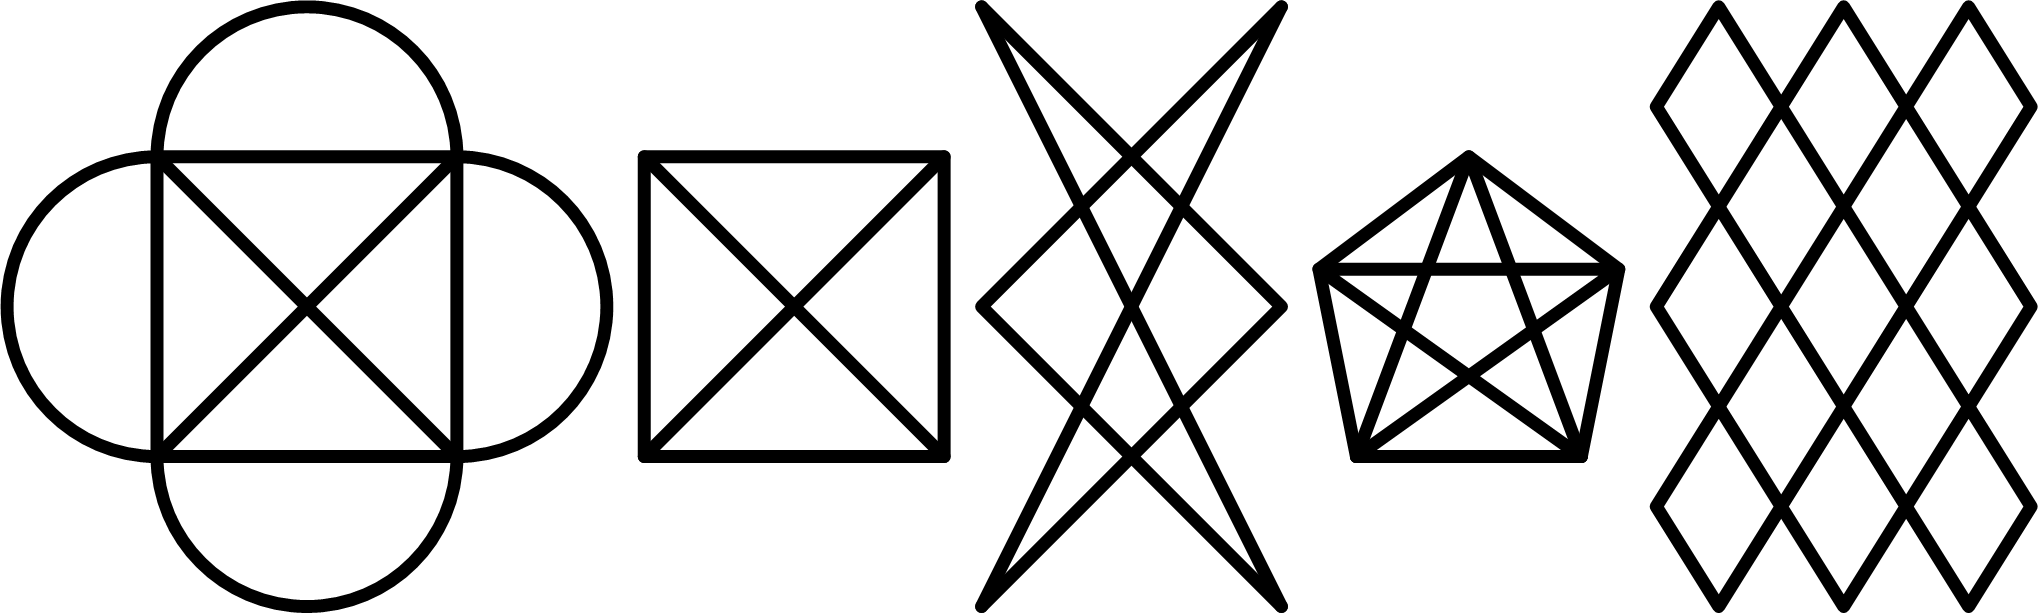
\includegraphics[width=0.7\textwidth]{fig/onlineFigure.png}
    \]
    
    \item Вычертить фигуру одним росчерком пера. При этом не обязательно маршрут, проходящий по всем ребрам, должен быть циклом, но пересекать ранее проведенную линию нельзя (как и проводить линию дважды). Доказать, что такой маршрут сущетвует, если все вершины имеют четную степень или, что только две вершины имеют нечетную степень.
    \[
        \begin{tabular}{ccccccccc}
            {\xymatrix{
                *{} \ar@{-}[r] \ar@{-}[dr] \ar@{-}[d]
                    &*{} \ar@{-}[d] \ar@{-}[dl] \ar@{-}@/^/[d]
                        \\
                *{} \ar@{-}[r]
                    &*{}                    
            }}
            &
            &
            {\xymatrix{
                *{} \ar@{-}[r] \ar@{-}@/^/[r] \ar@{-}@/_/[d] \ar@{-}[dr] \ar@{-}[d]
                    &*{} \ar@{-}[d] \ar@{-}[dl] \ar@{-}@/^/[d]
                        \\
                *{} \ar@{-}[r]
                    &*{}                    
            }}
            &
            &
            {\xymatrix{
                *{} \ar@{-}[r] \ar@{-}@/_/[d] \ar@{-}[d]
                    &*{} \ar@{-}[d] \ar@{-}@/^/[d]
                        \\
                *{} \ar@{-}[r]
                    &*{}                    
            }}
            &
            &
            {\xymatrix{
                *{} \ar@{-}[r] \ar@{-}@/_/[d] \ar@{-}[dr] \ar@{-}[d]
                    &*{} \ar@{-}[d] \ar@{-}@/^/[d]
                        \\
                *{} \ar@{-}[r]
                    &*{}                    
            }}
            &
            &
            {\xymatrix{
                *{} \ar@{-}[r] \ar@{-}@/^/[r] \ar@{-}[d] \ar@{-}[dr]
                    &*{} \ar@{-}[r] \ar@{-}[d] \ar@{-}[dr] \ar@{-}[dl]
                        &*{} \ar@{-}[d] \ar@{-}[dl]
                            \\
                *{} \ar@{-}[r]
                    &*{} \ar@{-}[r] \ar@{-}@/_/[r]
                        &*{} 
            }}
        \end{tabular}
    \]
    
    \item Найти гамильтоновы циклы в графах
    \[
        \begin{tabular}{cc}
            {
                \shorthandoff{"}
                \raisebox{\height}{
                    \(
                        \begin{xy}
                            \POS (0.00,15.00)*+[o][F-]{a}="a1"           \POS (14.27,4.64)*+[o][F-]{b}="b1"
                            \POS (8.82,-12.14)*+[o][F-]{c}="c1"          \POS (-8.82,-12.14)*+[o][F-]{d}="d1"
                            \POS (-14.27,4.64)*+[o][F-]{e}="e1"          \POS (0.00,7.00)*+[o][F-]{f}="a2"
                            \POS (6.66,2.16)*+[o][F-]{g}="b2"            \POS (4.11,-5.66)*+[o][F-]{h}="c2"
                            \POS (-4.11,-5.66)*+[o][F-]{i}="d2"          \POS (-6.66,2.16)*+[o][F-]{j}="e2"
                            \POS"a1" \ar @{-} "b1"            \POS"b1" \ar @{-} "c1"
                            \POS"c1" \ar @{-} "d1"            \POS"d1" \ar @{-} "e1"
                            \POS"e1" \ar @{-} "a1"            \POS"a2" \ar @{-} "b2"
                            \POS"b2" \ar @{-} "c2"            \POS"c2" \ar @{-} "d2"
                            \POS"d2" \ar @{-} "e2"            \POS"e2" \ar @{-} "a2"
                            \POS"a1" \ar @{-} "a2"            \POS"b1" \ar @{-} "b2"
                            \POS"c1" \ar @{-} "c2"            \POS"d1" \ar @{-} "d2"
                            \POS"e1" \ar @{-} "e2" 
                        \end{xy}        
                    \) 
                }
                \shorthandon{"}            
            }
            &
            \(\shorthandoff{"}
                \begin{xy}
                    \POS (0.00,40.00)*+[o][F-]{a}="l0"        \POS (0.00,28.57)*+[o][F-]{b}="l1"
                    \POS (9.38,22.86)*+[o][F-]{c}="l2"        \POS (18.75,22.86)*+[o][F-]{d}="l3"
                    \POS (25.00,28.57)*+[o][F-]{e}="l4"       \POS (25.00,17.14)*+[o][F-]{f}="l5"
                    \POS (6.25,11.43)*+[o][F-]{g}="l6"        \POS (9.38,0.00)*+[o][F-]{h}="l7"
                    \POS (-9.38,22.86)*+[o][F-]{i}="l8"       \POS (-18.75,22.86)*+[o][F-]{j}="l9"
                    \POS (-25.00,28.57)*+[o][F-]{k}="l10"     \POS (-25.00,17.14)*+[o][F-]{l}="l11"
                    \POS (-6.25,11.43)*+[o][F-]{m}="l12"      \POS (-9.38,0.00)*+[o][F-]{n}="l13"        
                    \POS "l0" \ar @{-} "l1"        \POS "l12" \ar @{-} "l6"
                    \POS "l13" \ar @{-} "l7"       \POS "l0" \ar @{-} "l4"
                    \POS "l0" \ar @{-} "l10"       \POS "l4" \ar @{-} "l5"
                    \POS "l10" \ar @{-} "l11"      \POS "l4" \ar @{-} "l3"
                    \POS "l10" \ar @{-} "l9"       \POS "l5" \ar @{-} "l3"
                    \POS "l11" \ar @{-} "l9"       \POS "l2" \ar @{-} "l3"
                    \POS "l8" \ar @{-} "l9"        \POS "l1" \ar @{-} "l2"
                    \POS "l1" \ar @{-} "l8"        \POS "l2" \ar @{-} "l6"
                    \POS "l8" \ar @{-} "l12"       \POS "l5" \ar @{-} "l7"
                    \POS "l11" \ar @{-} "l13"      \POS "l6" \ar @{-} "l7"
                    \POS "l12" \ar @{-} "l13"
                \end{xy}
                \shorthandon{"}            
            \)
        \end{tabular}
    \]

    \item Найти гамильтонов цикл в графе на рис. \ref{fig:graph:gamilton}.
    
    \item Найти изоморфизм графов
    \begin{enumerate}
        \item
        \(
            \shorthandoff{"}
            \begin{xy}
                \POS (0.00,15.00)*+[o][F-]{1}="a1"    \POS (11.73,9.35)*+[o][F-]{2}="b1"
                \POS (14.62,-3.34)*+[o][F-]{3}="c1"   \POS (6.51,-13.51)*+[o][F-]{4}="d1"
                \POS (-6.51,-13.51)*+[o][F-]{5}="e1"  \POS (-14.62,-3.34)*+[o][F-]{6}="f1"
                \POS (-11.73,9.35)*+[o][F-]{7}="g1"   \POS (40.00,15.00)*+[o][F-]{a}="a2"
                \POS (51.73,9.35)*+[o][F-]{b}="b2"    \POS (54.62,-3.34)*+[o][F-]{c}="c2"
                \POS (46.51,-13.51)*+[o][F-]{d}="d2"  \POS (33.49,-13.51)*+[o][F-]{e}="e2"
                \POS (25.38,-3.34)*+[o][F-]{f}="f2"   \POS (28.27,9.35)*+[o][F-]{g}="g2"
                \POS"a1" \ar @{-} "b1"    \POS"a1" \ar @{-} "c1"
                \POS"a1" \ar @{-} "f1"    \POS"a1" \ar @{-} "g1"
                \POS"b1" \ar @{-} "g1"    \POS"b1" \ar @{-} "c1"
                \POS"b1" \ar @{-} "d1"    \POS"c1" \ar @{-} "d1"
                \POS"c1" \ar @{-} "e1"    \POS"d1" \ar @{-} "e1"
                \POS"d1" \ar @{-} "f1"    \POS"e1" \ar @{-} "f1"
                \POS"e1" \ar @{-} "g1"    \POS"f1" \ar @{-} "g1"
                \POS"a2" \ar @{-} "b2"    \POS"a2" \ar @{-} "d2"
                \POS"b2" \ar @{-} "c2"    \POS"b2" \ar @{-} "e2"
                \POS"c2" \ar @{-} "d2"    \POS"c2" \ar @{-} "f2"
                \POS"d2" \ar @{-} "e2"    \POS"d2" \ar @{-} "g2"
                \POS"e2" \ar @{-} "f2"    \POS"e2" \ar @{-} "a2"
                \POS"f2" \ar @{-} "g2"    \POS"f2" \ar @{-} "b2"
                \POS"g2" \ar @{-} "a2"    \POS"g2" \ar @{-} "c2" 
            \end{xy}
            \shorthandon{"}
        \)
        \item
        \begin{tabular}{cc}
            {\entrymodifiers={+[o][F-]}
            \xymatrix@=6pt{
                a \ar@{-}[ddd] \ar@{-}[ddr] \ar@{-}[dr] \ar@{-}@/^21pt/[dddrrr]
                    &*{}
                        &*{}
                            &*{}
                                \\
                *{}
                    &b \ar@{-}[d] \ar@{-}[dr]
                        &*{}
                            &*{}
                                \\
                *{}
                    &n \ar@{-}[dl] \ar@{-}[drr]
                        &c \ar@{-}[dr]
                            &*{}
                                \\
                e \ar@{-}[rrr]
                    &*{}
                        &*{}
                            &d
            }}
            &
            {\entrymodifiers={+[o][F-]}
            \xymatrix@=6pt{
                1 \ar@{-}[dd] \ar@{-}[rr]  \ar@{-}[dr]
                    &*{}
                        &2 \ar@{-}[dr] \ar@{-}[dd] \ar@{-}[dl]
                            &*{}
                                \\
                *{}
                    &3 \ar@{-}[rr] \ar@{-}[dr] \ar@{-}[dl]
                        &*{}
                            &4 \ar@{-}[dl]
                                \\
                5 \ar@{-}[rr]
                    &*{}
                        &6
                            &*{}
            }}
        \end{tabular}
        
        \item
        \begin{tabular}{cc}
            {\entrymodifiers={+[o][F-]}
            \xymatrix@=6pt{
                1 \ar@{-}[dd] \ar@{-}[ddrr] \ar@{-}[rr]
                    &*{}
                        &2 \ar@{-}[ddll] \ar@{-}[dr] \ar@{-}[dr]  \ar@{-}[dd]
                            &*{}
                                \\
                *{}
                    &*{}
                        &*{}
                            &3 \ar@{-}[dl]
                                \\
                5
                    &*{}
                        &4 \ar@{-}[ll]
                            &*{}
            }}
            &
            {\entrymodifiers={+[o][F-]}
            \xymatrix@=6pt{
                a \ar@{-}[dd] \ar@{-}[ddrr] \ar@{-}[rr] \ar@{-}[drrr]
                    &*{}
                        &b \ar@{-}[ddll] \ar@{-}[dd]
                            &*{}
                                \\
                *{}
                    &*{}
                        &*{}
                            &c \ar@{-}[dl]
                                \\
                e
                    &*{}
                        &d \ar@{-}[ll]
                            &*{}
            }}
        \end{tabular}
    \end{enumerate}
    
    \item Выполнить укладку графов на плоскости
    \[
        \begin{tabular}{ccc}
            {
                \shorthandoff{"}
                \begin{xy}
                    \POS (0.00,15.00)*++[o][F-]{1}="a1"
                    \POS (14.27,4.64)*++[o][F-]{2}="b1"
                    \POS (8.82,-12.14)*++[o][F-]{3}="c1"
                    \POS (-8.82,-12.14)*++[o][F-]{4}="d1"
                    \POS (-14.27,4.64)*++[o][F-]{5}="e1"
                    \POS"a1" \ar @{-} "b1"
                    \POS"a1" \ar @{-} "c1"
                    \POS"a1" \ar @{-} "d1"
                    \POS"a1" \ar @{-} "e1"
                    \POS"b1" \ar @{-} "c1"
                    \POS"b1" \ar @{-} "d1"
                    \POS"b1" \ar @{-} "e1"
                    \POS"c1" \ar @{-} "e1"
                    \POS"d1" \ar @{-} "e1"
                \end{xy}        
                \shorthandon{"}            
            }        
            &
            \raisebox{1.5\height}{
                {\xymatrix{
                    1 \ar@{-}[d] \ar@{-}[dr] \ar@{-}[r]
                        &2 \ar@{-}[dl] \ar@{-}[d] \ar@{-}[dr] \ar@{-}[r]
                            &3 \ar@{-}[dll] \ar@{-}[dl] \ar@{-}[d]
                                \\
                    4 \ar@{-}[r]
                        &5 \ar@{-}[r]
                            &6                        
                }}
            }
            &
            {
                \shorthandoff{"}
                \begin{xy}
                    \POS (0.00,15.00)*++[o][F-]{1}="a2"
                    \POS (11.73,9.35)*++[o][F-]{2}="b2"
                    \POS (14.62,-3.34)*++[o][F-]{3}="c2"
                    \POS (6.51,-13.51)*++[o][F-]{4}="d2"
                    \POS (-6.51,-13.51)*++[o][F-]{5}="e2"
                    \POS (-14.62,-3.34)*++[o][F-]{6}="f2"
                    \POS (-11.73,9.35)*++[o][F-]{7}="g2"
                    \POS"a2" \ar @{-} "b2"
                    \POS"a2" \ar @{-} "d2"
                    \POS"b2" \ar @{-} "c2"
                    \POS"b2" \ar @{-} "e2"
                    \POS"c2" \ar @{-} "d2"
                    \POS"c2" \ar @{-} "f2"
                    \POS"d2" \ar @{-} "g2"
                    \POS"e2" \ar @{-} "f2"
                    \POS"e2" \ar @{-} "a2"
                    \POS"f2" \ar @{-} "g2"
                    \POS"f2" \ar @{-} "b2"
                    \POS"g2" \ar @{-} "a2"
                    \POS"g2" \ar @{-} "c2" 
                \end{xy}
                \shorthandon{"}
            }
        \end{tabular}
    \]
    
    \item Определите цикломатические числа в приведенных графах. Сколько всего циклов можно выделить в этих графах? Выделите цикловой базис, разложите все возможные циклы в этом базисе.
    
    \begin{tabular}{ccc}
        \(    
            {\xymatrix{
                1 \ar@{-}[d] \ar@{-}[dr] \ar@{-}[r]
                    &2 \ar@{-}[dl] \ar@{-}[d]
                        \\
                4 \ar@{-}[r]
                    &3 
            }}
        \)   
        &        
        \(    
            {\xymatrix@=7pt{
                1 \ar@{-}[dd] \ar@{-}[dr] \ar@{-}[rr]
                    &*{}
                        &2 \ar@{-}[dl] \ar@{-}[dd]
                            \\
                *{}
                    &5 \ar@{-}[dr]
                        &*{}
                            \\
                4 \ar@{-}[rr]
                    &*{}
                        &3 
            }}
        \)
        &
        \(    
            {\xymatrix@=7pt{
                1 \ar@{-}[dd] \ar@{-}[dr] \ar@{-}[rr]
                    &*{}
                        &2 \ar@{-}[dl] \ar@{-}[dd]
                            \\
                *{}
                    &5 \ar@{-}[dr] \ar@{-}[dl]
                        &*{}
                            \\
                4 \ar@{-}[rr]
                    &*{}
                        &3 
            }}
        \)
    \end{tabular}
    
\end{enumerate}
